\section{Experiments}

%  ————————————————————————————————————————————————————————————————————————————————旧版数据
% % \documentclass{article}
% % \usepackage{graphicx}
% % \usepackage{multirow}
% % \usepackage{booktabs}
% % \usepackage[table]{xcolor}
% % \usepackage{rotating}
% % \usepackage{adjustbox}

% % \begin{document}

% \begin{table*}[t]
% % \caption{Main Results on LongBench: performance comparison of different KV cache compression methods across 13 datasets on three models (Llama3-8B-Instruct, Qwen2.5-7B-Instruct, Qwen3-8B) under cache sizes of 256, 128, and 64, with complete results available in Appendix \ref{Complete Experiment Results on LongBench}.}
% \centering
% \small
% \resizebox{\textwidth}{!}{%
% \begin{tabular}{>{\bfseries}c >{\raggedright}p{1.2cm} *{14}{c}}
% \toprule
% &  & \multicolumn{2}{c}{\textbf{Single-Document QA}} & \multicolumn{2}{c}{\textbf{Multi-Document QA}} & \multicolumn{2}{c}{\textbf{Summarization}} & \multicolumn{3}{c}{\textbf{Few-shot Learning}} & \multicolumn{2}{c}{\textbf{Synthetic}} & \multicolumn{2}{c}{\textbf{Code}} &  \\
% \cmidrule(lr){3-4}\cmidrule(lr){5-6}\cmidrule(lr){7-8}\cmidrule(lr){9-11}\cmidrule(lr){12-13}\cmidrule(lr){14-15}
% & \textbf{Methods} & \rotatebox[origin=c]{30}{\textbf{Qasper}} & \rotatebox[origin=c]{30}{\textbf{MF-en}} & \rotatebox[origin=c]{30}{\textbf{HotpotQA}} & \rotatebox[origin=c]{30}{\textbf{2WikiMQA}} & \rotatebox[origin=c]{30}{\textbf{GovReport}} & \rotatebox[origin=c]{30}{\textbf{MultiNews}} & \rotatebox[origin=c]{30}{\textbf{TREC}} & \rotatebox[origin=c]{30}{\textbf{TriviaQA}} & \rotatebox[origin=c]{30}{\textbf{SAMSum}} & \rotatebox[origin=c]{30}{\textbf{PCount}} & \rotatebox[origin=c]{30}{\textbf{PRe}} & \rotatebox[origin=c]{30}{\textbf{Lcc}} & \rotatebox[origin=c]{30}{\textbf{RB-P}} & \textbf{Avg.} \\
% \midrule
% & FullKV & 37.68 & 40.56 & 50.14 & 34.93 & 30.99 & 25.62 & 70.00 & 89.85 & 40.50 & 13.28 & 83.67 & 56.44 & 50.97 & 48.05 \\
% & \multicolumn{15}{c}{\cellcolor{gray!20}\textbf{KV Cache Size = 256}} \\
% \multirow{13}{*}{\rotatebox{90}{Llama3-8B-Instruct}} & H2O & 28.11 & 36.63 & 48.62 & 31.50 & 21.87 & 21.44 & 45.67 & 89.49 & 38.28 & 12.11 & 83.67 & 61.49 & 53.36 & 44.02 \\
% & PyramidKV & 30.88 & 38.11 & 50.20 & 33.88 & \textbf{22.54} & 21.84 & 60.00 & 89.26 & 37.07 & \textbf{12.78} & 83.67 & 61.34 & 52.51 & 45.70 \\
% & SnapKV & 30.84 & \textbf{38.39} & 49.75 & 33.80 & 22.18 & 21.53 & 57.00 & 89.65 & 36.97 & 12.11 & \textbf{84.00} & 61.78 & 54.92 & 45.61 \\
% & DapQ & \textbf{32.55} & 38.18 & \textbf{50.67} & \textbf{34.35} & 22.25 & \textbf{21.89} & \textbf{60.67} & \textbf{90.48} & \textbf{38.34} & 11.78 & 83.67 & \textbf{62.78} & \textbf{55.64} & \textbf{46.40} \\
% & \multicolumn{15}{c}{\cellcolor{gray!20}\textbf{KV Cache Size = 128}} \\
% & H2O & 25.95 & 36.25 & 48.65 & 31.90 & \textbf{20.79} & 20.30 & 40.00 & 87.29 & 36.25 & 12.33 & \textbf{83.67} & 59.81 & 53.14 & 42.79 \\
% & PyramidKV & 28.80 & \textbf{38.29} & 49.52 & 31.60 & 20.67 & 20.55 & 49.00 & 87.68 & 36.73 & \textbf{12.44} & 82.00 & 60.36 & 52.03 & 43.82 \\
% & SnapKV & \textbf{29.52} & 37.80 & 49.36 & 32.40 & 19.87 & 20.08 & 47.67 & 87.82 & 35.63 & 11.44 & 82.33 & 61.49 & 52.40 & 43.68 \\
% & DapQ & 28.76 & 37.24 & \textbf{50.04} & \textbf{33.59} & 20.47 & \textbf{20.63} & \textbf{50.00} & \textbf{90.06} & \textbf{36.87} & 12.11 & 81.67 & \textbf{61.81} & \textbf{53.92} & \textbf{44.40} \\
% & \multicolumn{15}{c}{\cellcolor{gray!20}\textbf{KV Cache Size = 64}} \\
% & H2O & 24.02 & 30.83 & 48.27 & 31.70 & \textbf{19.37} & \textbf{19.14} & 37.33 & 86.27 & 35.18 & 7.72 & \textbf{82.33} & 59.20 & \textbf{51.10} & 40.96 \\
% & PyramidKV & 22.04 & 31.80 & 47.01 & 31.54 & 15.70 & 16.34 & 39.00 & 76.80 & 32.31 & 10.33 & 79.67 & 55.19 & 47.90 & 38.90 \\
% & SnapKV & 25.06 & 32.92 & 47.16 & 31.71 & 16.85 & 17.09 & \textbf{40.67} & 86.02 & 33.99 & 11.78 & 78.00 & 57.95 & 50.91 & 40.78 \\
% & DapQ & \textbf{25.99} & \textbf{37.36} & \textbf{49.11} & \textbf{32.88} & 18.46 & 18.70 & 38.67 & \textbf{87.38} & \textbf{35.30} & \textbf{11.89} & 77.67 & \textbf{60.19} & 49.90 & \textbf{41.81} \\
% \midrule
% % & FullKV & 36.50 & 49.70 & 55.91 & 44.70 & 31.64 & 22.84 & 66.33 & 89.34 & 42.49 & 11.00 & 86.33 & 61.97 & 59.97 & 50.67 \\
% % & \multicolumn{15}{c}{\cellcolor{gray!20}\textbf{KV Cache Size = 256}} \\
% % \multirow{12}{*}{\rotatebox{90}{Qwen2.5-7B-Instruct}} & H2O & 27.76 & 42.94 & 47.89 & 40.97 & 22.13 & 18.31 & 44.33 & 84.51 & 39.77 & 10.67 & 86.00 & 57.07 & 54.09 & 44.31 \\
% % & PyramidKV & 29.65 & 46.37 & 49.89 & 40.77 & 20.42 & 16.80 & 53.00 & 87.89 & 39.61 & 10.67 & 86.00 & 52.61 & 49.49 & 44.82 \\
% % & SnapKV & \textbf{31.12} & \textbf{47.87} & 51.76 & 40.78 & 22.25 & \textbf{18.41} & 53.33 & 87.66 & 39.34 & 10.67 & 86.00 & 56.87 & \textbf{54.36} & 46.19 \\
% % & DapQ & 30.21 & 45.00 & \textbf{51.92} & \textbf{41.46} & \textbf{22.35} & 18.40 & \textbf{56.67} & \textbf{88.64} & \textbf{39.92} & \textbf{11.00} & \textbf{86.00} & \textbf{58.40} & 53.82 & \textbf{46.45} \\
% % & \multicolumn{15}{c}{\cellcolor{gray!20}\textbf{KV Cache Size = 128}} \\
% % & H2O & 26.83 & 37.80 & 45.14 & 39.77 & \textbf{20.13} & 16.64 & 40.67 & 81.43 & 38.56 & 10.67 & \textbf{85.67} & 53.97 & 51.52 & 42.22 \\
% % & PyramidKV & 26.37 & 43.09 & 46.57 & 39.07 & 18.01 & 15.15 & 43.33 & 84.69 & 38.40 & 10.67 & 84.67 & 49.45 & 46.90 & 42.03 \\
% % & SnapKV & \textbf{27.46} & 41.81 & 48.62 & 41.40 & 19.42 & 16.19 & 42.33 & 83.91 & \textbf{38.89} & 10.67 & 85.00 & 52.14 & 51.39 & 43.02 \\
% % & DapQ & 26.81 & \textbf{43.12} & \textbf{49.62} & \textbf{41.36} & 19.89 & \textbf{16.68} & \textbf{47.00} & \textbf{84.92} & 38.07 & \textbf{11.00} & 85.00 & \textbf{54.46} & \textbf{51.70} & \textbf{43.82} \\
% % & \multicolumn{15}{c}{\cellcolor{gray!20}\textbf{KV Cache Size = 64}} \\
% % & H2O & 24.33 & 32.36 & 44.94 & 39.06 & \textbf{17.96} & \textbf{15.05} & 37.33 & 82.76 & 35.27 & 10.67 & \textbf{85.00} & \textbf{49.44} & 45.52 & 39.98 \\
% % & PyramidKV & 22.36 & 35.19 & 43.51 & 38.08 & 14.04 & 11.10 & 37.33 & 84.81 & 35.58 & 10.67 & 80.33 & 44.67 & 42.22 & 38.45 \\
% % & SnapKV & 22.90 & 40.66 & 45.56 & 40.28 & 15.42 & 12.03 & 37.67 & \textbf{85.11} & 36.92 & 10.67 & 82.00 & 46.16 & 45.75 & 40.09 \\
% % & DapQ & \textbf{25.58} & \textbf{42.65} & \textbf{49.66} & \textbf{41.25} & 16.90 & 14.05 & \textbf{39.67} & 84.16 & \textbf{35.49} & \textbf{11.00} & 80.67 & 49.38 & \textbf{46.77} & \textbf{41.33} \\
% % % \midrule
% & FullKV & 36.87 & 53.67 & 57.67 & 44.73 & 33.39 & 23.69 & 71.67 & 91.79 & 42.07 & 11.98 & 86.67 & 70.64 & 59.26 & 52.60 \\
% & \multicolumn{15}{c}{\cellcolor{gray!20}\textbf{KV Cache Size = 256}} \\
% \multirow{12}{*}{\rotatebox{90}{Qwen3-8B}} & H2O & 27.80 & 44.92 & 51.37 & 40.50 & 22.38 & 18.26 & 46.33 & 90.04 & 38.98 & 12.33 & 86.67 & 66.11 & 53.93 & 46.12 \\
% & PyramidKV & 30.41 & 47.81 & 51.00 & 41.37 & 22.36 & 17.41 & 61.67 & 90.96 & 37.65 & 13.00 & 86.33 & 67.01 & 50.11 & 47.47 \\
% & SnapKV & \textbf{32.40} & 49.29 & 54.38 & 41.40 & 23.79 & 18.99 & \textbf{63.00} & 91.07 & 38.57 & \textbf{14.67} & 86.67 & \textbf{67.99} & 53.77 & 48.92 \\
% & DapQ & 32.14 & \textbf{50.78} & \textbf{54.79} & \textbf{44.47} & \textbf{24.16} & \textbf{19.01} & 62.67 & \textbf{91.15} & \textbf{39.61} & 14.17 & \textbf{86.67} & 67.20 & \textbf{53.83} & \textbf{49.28} \\
% & \multicolumn{15}{c}{\cellcolor{gray!20}\textbf{KV Cache Size = 128}} \\
% & H2O & 26.60 & 41.37 & 48.10 & 39.85 & 20.83 & 17.27 & 41.33 & 90.21 & 38.16 & \textbf{11.72} & \textbf{86.67} & 65.22 & 52.77 & 44.22 \\
% & PyramidKV & 26.22 & 40.48 & 48.41 & 39.46 & 18.99 & 15.10 & 48.33 & 89.31 & 36.92 & 9.67 & 86.67 & 60.82 & 48.78 & 43.78 \\
% & SnapKV & \textbf{29.41} & 46.43 & 51.20 & 41.66 & 20.37 & 16.64 & 51.33 & \textbf{91.07} & 37.37 & 11.00 & 86.67 & 65.36 & 51.65 & 46.17 \\
% & DapQ & 29.10 & \textbf{47.15} & \textbf{53.84} & \textbf{43.00} & \textbf{21.11} & \textbf{17.27} & \textbf{54.00} & 90.45 & \textbf{38.50} & 11.67 & 86.00 & \textbf{66.29} & \textbf{52.03} & \textbf{46.95} \\
% & \multicolumn{15}{c}{\cellcolor{gray!20}\textbf{KV Cache Size = 64}} \\
% & H2O & 25.55 & 38.94 & 46.66 & 39.27 & \textbf{18.55} & \textbf{15.23} & 39.00 & 88.13 & 35.98 & 9.67 & \textbf{86.67} & 59.48 & \textbf{48.95} & 42.47 \\
% & PyramidKV & 25.32 & 40.44 & 46.61 & 39.20 & 16.25 & 12.93 & \textbf{44.67} & 88.27 & 34.63 & 11.33 & 83.67 & 59.73 & 46.48 & 42.27 \\
% & SnapKV & 25.09 & 39.89 & 46.58 & 39.38 & 15.28 & 12.38 & 42.67 & 87.93 & 35.12 & 11.33 & 84.33 & 57.96 & 46.49 & 41.88 \\
% & DapQ & \textbf{25.78} & \textbf{43.17} & \textbf{49.84} & \textbf{41.28} & 17.16 & 13.95 & 43.00 & \textbf{88.97} & \textbf{36.00} & \textbf{12.67} & 83.00 & \textbf{60.31} & 46.90 & \textbf{43.23} \\
% \bottomrule
% \end{tabular}
% }
% \vspace{-9pt}
% \caption{Main Results on LongBench: performance comparison of different KV cache compression methods}
% \vspace{-12pt}
% \label{table:longbench}
% \end{table*}

% % \end{document}


%  ————————————————————————————————————————————————————————————————————————————————更新的新版数据


% \documentclass{article}
% \usepackage{graphicx}
% \usepackage{multirow}
% \usepackage{booktabs}
% \usepackage[table]{xcolor}
% \usepackage{rotating}
% \usepackage{adjustbox}

% \begin{document}

\begin{table*}[t]
% \caption{Main Results on LongBench: performance comparison of different KV cache compression methods across 13 datasets on three models (Llama3-8B-Instruct, Qwen2.5-7B-Instruct, Qwen3-8B) under cache sizes of 256, 128, and 64, with complete results available in Appendix \ref{Complete Experiment Results on LongBench}.}
\centering
\small
\resizebox{\textwidth}{!}{%
\begin{tabular}{>{\bfseries}c >{\raggedright}p{1.2cm} *{14}{c}}
\toprule
&  & \multicolumn{2}{c}{\textbf{Single-Document QA}} & \multicolumn{2}{c}{\textbf{Multi-Document QA}} & \multicolumn{2}{c}{\textbf{Summarization}} & \multicolumn{3}{c}{\textbf{Few-shot Learning}} & \multicolumn{2}{c}{\textbf{Synthetic}} & \multicolumn{2}{c}{\textbf{Code}} &  \\
\cmidrule(lr){3-4}\cmidrule(lr){5-6}\cmidrule(lr){7-8}\cmidrule(lr){9-11}\cmidrule(lr){12-13}\cmidrule(lr){14-15}
& \textbf{Methods} & \rotatebox[origin=c]{30}{\textbf{Qasper}} & \rotatebox[origin=c]{30}{\textbf{MF-en}} & \rotatebox[origin=c]{30}{\textbf{HotpotQA}} & \rotatebox[origin=c]{30}{\textbf{2WikiMQA}} & \rotatebox[origin=c]{30}{\textbf{GovReport}} & \rotatebox[origin=c]{30}{\textbf{MultiNews}} & \rotatebox[origin=c]{30}{\textbf{TREC}} & \rotatebox[origin=c]{30}{\textbf{TriviaQA}} & \rotatebox[origin=c]{30}{\textbf{SAMSum}} & \rotatebox[origin=c]{30}{\textbf{PCount}} & \rotatebox[origin=c]{30}{\textbf{PRe}} & \rotatebox[origin=c]{30}{\textbf{Lcc}} & \rotatebox[origin=c]{30}{\textbf{RB-P}} & \textbf{Avg.} \\
\midrule
& FullKV & 37.72 & 40.64 & 50.17 & 34.88 & 31.03 & 25.64 & 70.00 & 89.85 & 40.55 & 13.30 & 83.67 & 58.96 & 52.71 & 48.39 \\
& \multicolumn{15}{c}{\cellcolor{gray!20}\textbf{KV Cache Size = 256}} \\
\multirow{13}{*}{\rotatebox{90}{Llama3-8B-Instruct}} & H2O & 28.11 & 36.63 & 48.62 & 31.50 & 21.87 & 21.44 & 45.67 & 89.49 & 38.28 & 12.11 & 83.67 & 61.49 & 53.36 & 44.02 \\
& PyramidKV & 30.88 & 38.11 & 50.20 & 33.88 & \textbf{22.54} & 21.84 & 60.00 & 89.26 & 37.07 & \textbf{12.78} & 83.67 & 61.34 & 52.51 & 45.70 \\
& SnapKV & 30.84 & \textbf{38.39} & 49.75 & 33.80 & 22.18 & 21.53 & 57.00 & 89.65 & 36.97 & 12.11 & \textbf{84.00} & 61.78 & 54.92 & 45.61 \\
& DapQ & \textbf{32.55} & 38.18 & \textbf{50.67} & \textbf{34.35} & 22.25 & \textbf{21.89} & \textbf{60.67} & \textbf{90.48} & \textbf{38.34} & 11.78 & 83.67 & \textbf{62.78} & \textbf{55.64} & \textbf{46.40} \\
& \multicolumn{15}{c}{\cellcolor{gray!20}\textbf{KV Cache Size = 128}} \\
& H2O & 25.95 & 36.25 & 48.65 & 31.90 & \textbf{20.79} & 20.30 & 40.00 & 87.29 & 36.25 & 12.33 & \textbf{83.67} & 59.81 & 53.14 & 42.79 \\
& PyramidKV & 28.80 & \textbf{38.29} & 49.52 & 31.60 & 20.67 & 20.55 & 49.00 & 87.68 & 36.73 & \textbf{12.44} & 82.00 & 60.36 & 52.03 & 43.82 \\
& SnapKV & \textbf{29.52} & 37.80 & 49.36 & 32.40 & 19.87 & 20.08 & 47.67 & 87.82 & 35.63 & 11.44 & 82.33 & 61.49 & 52.40 & 43.68 \\
& DapQ & 28.76 & 37.24 & \textbf{50.04} & \textbf{33.59} & 20.47 & \textbf{20.63} & \textbf{50.00} & \textbf{90.06} & \textbf{36.87} & 12.11 & 81.67 & \textbf{61.81} & \textbf{53.92} & \textbf{44.40} \\
& \multicolumn{15}{c}{\cellcolor{gray!20}\textbf{KV Cache Size = 64}} \\
& H2O & 24.02 & 30.83 & 48.27 & 31.70 & \textbf{19.37} & \textbf{19.14} & 37.33 & 86.27 & 35.18 & 7.72 & \textbf{82.33} & 59.20 & \textbf{51.10} & 40.96 \\
& PyramidKV & 22.04 & 31.80 & 47.01 & 31.54 & 15.70 & 16.34 & 39.00 & 76.80 & 32.31 & 10.33 & 79.67 & 55.19 & 47.90 & 38.90 \\
& SnapKV & 25.06 & 32.92 & 47.16 & 31.71 & 16.85 & 17.09 & \textbf{40.67} & 86.02 & 33.99 & 11.78 & 78.00 & 57.95 & 50.91 & 40.78 \\
& DapQ & \textbf{25.99} & \textbf{37.36} & \textbf{49.11} & \textbf{32.88} & 18.46 & 18.70 & 38.67 & \textbf{87.38} & \textbf{35.30} & \textbf{11.89} & 77.67 & \textbf{60.19} & 49.90 & \textbf{41.81} \\
\midrule
% & FullKV & 36.50 & 49.70 & 55.91 & 44.70 & 31.64 & 22.84 & 66.33 & 89.34 & 42.49 & 11.00 & 86.33 & 61.97 & 59.97 & 50.67 \\
% & \multicolumn{15}{c}{\cellcolor{gray!20}\textbf{KV Cache Size = 256}} \\
% \multirow{12}{*}{\rotatebox{90}{Qwen2.5-7B-Instruct}} & H2O & 27.76 & 42.94 & 47.89 & 40.97 & 22.13 & 18.31 & 44.33 & 84.51 & 39.77 & 10.67 & 86.00 & 57.07 & 54.09 & 44.31 \\
% & PyramidKV & 29.65 & 46.37 & 49.89 & 40.77 & 20.42 & 16.80 & 53.00 & 87.89 & 39.61 & 10.67 & 86.00 & 52.61 & 49.49 & 44.82 \\
% & SnapKV & \textbf{31.12} & \textbf{47.87} & 51.76 & 40.78 & 22.25 & \textbf{18.41} & 53.33 & 87.66 & 39.34 & 10.67 & 86.00 & 56.87 & \textbf{54.36} & 46.19 \\
% & DapQ & 30.21 & 45.00 & \textbf{51.92} & \textbf{41.46} & \textbf{22.35} & 18.40 & \textbf{56.67} & \textbf{88.64} & \textbf{39.92} & \textbf{11.00} & \textbf{86.00} & \textbf{58.40} & 53.82 & \textbf{46.45} \\
% & \multicolumn{15}{c}{\cellcolor{gray!20}\textbf{KV Cache Size = 128}} \\
% & H2O & 26.83 & 37.80 & 45.14 & 39.77 & \textbf{20.13} & 16.64 & 40.67 & 81.43 & 38.56 & 10.67 & \textbf{85.67} & 53.97 & 51.52 & 42.22 \\
% & PyramidKV & 26.37 & 43.09 & 46.57 & 39.07 & 18.01 & 15.15 & 43.33 & 84.69 & 38.40 & 10.67 & 84.67 & 49.45 & 46.90 & 42.03 \\
% & SnapKV & \textbf{27.46} & 41.81 & 48.62 & 41.40 & 19.42 & 16.19 & 42.33 & 83.91 & \textbf{38.89} & 10.67 & 85.00 & 52.14 & 51.39 & 43.02 \\
% & DapQ & 26.81 & \textbf{43.12} & \textbf{49.62} & \textbf{41.36} & 19.89 & \textbf{16.68} & \textbf{47.00} & \textbf{84.92} & 38.07 & \textbf{11.00} & 85.00 & \textbf{54.46} & \textbf{51.70} & \textbf{43.82} \\
% & \multicolumn{15}{c}{\cellcolor{gray!20}\textbf{KV Cache Size = 64}} \\
% & H2O & 24.33 & 32.36 & 44.94 & 39.06 & \textbf{17.96} & \textbf{15.05} & 37.33 & 82.76 & 35.27 & 10.67 & \textbf{85.00} & \textbf{49.44} & 45.52 & 39.98 \\
% & PyramidKV & 22.36 & 35.19 & 43.51 & 38.08 & 14.04 & 11.10 & 37.33 & 84.81 & 35.58 & 10.67 & 80.33 & 44.67 & 42.22 & 38.45 \\
% & SnapKV & 22.90 & 40.66 & 45.56 & 40.28 & 15.42 & 12.03 & 37.67 & \textbf{85.11} & 36.92 & 10.67 & 82.00 & 46.16 & 45.75 & 40.09 \\
% & DapQ & \textbf{25.58} & \textbf{42.65} & \textbf{49.66} & \textbf{41.25} & 16.90 & 14.05 & \textbf{39.67} & 84.16 & \textbf{35.49} & \textbf{11.00} & 80.67 & 49.38 & \textbf{46.77} & \textbf{41.33} \\
% % \midrule
& FullKV & 36.87 & 53.67 & 57.67 & 44.73 & 33.39 & 23.69 & 71.67 & 91.79 & 42.07 & 11.98 & 86.67 & 70.64 & 59.26 & 52.60 \\
& \multicolumn{15}{c}{\cellcolor{gray!20}\textbf{KV Cache Size = 256}} \\
\multirow{12}{*}{\rotatebox{90}{Qwen3-8B}} & H2O & 27.80 & 44.92 & 51.37 & 40.50 & 22.38 & 18.26 & 46.33 & 90.04 & 38.98 & 12.33 & 86.67 & 66.11 & 53.93 & 46.12 \\
& PyramidKV & 30.41 & 47.81 & 51.00 & 41.37 & 22.36 & 17.41 & 61.67 & 90.96 & 37.65 & 13.00 & 86.33 & 67.01 & 50.11 & 47.47 \\
& SnapKV & \textbf{32.40} & 49.29 & 54.38 & 41.40 & 23.79 & 18.99 & \textbf{63.00} & 91.07 & 38.57 & \textbf{14.67} & 86.67 & \textbf{67.99} & 53.77 & 48.92 \\
& DapQ & 32.14 & \textbf{50.78} & \textbf{54.79} & \textbf{44.47} & \textbf{24.16} & \textbf{19.01} & 62.67 & \textbf{91.15} & \textbf{39.61} & 14.17 & \textbf{86.67} & 67.20 & \textbf{53.83} & \textbf{49.28} \\
& \multicolumn{15}{c}{\cellcolor{gray!20}\textbf{KV Cache Size = 128}} \\
& H2O & 26.60 & 41.37 & 48.10 & 39.85 & 20.83 & 17.27 & 41.33 & 90.21 & 38.16 & \textbf{11.72} & \textbf{86.67} & 65.22 & 52.77 & 44.22 \\
& PyramidKV & 26.22 & 40.48 & 48.41 & 39.46 & 18.99 & 15.10 & 48.33 & 89.31 & 36.92 & 9.67 & 86.67 & 60.82 & 48.78 & 43.78 \\
& SnapKV & \textbf{29.41} & 46.43 & 51.20 & 41.66 & 20.37 & 16.64 & 51.33 & \textbf{91.07} & 37.37 & 11.00 & 86.67 & 65.36 & 51.65 & 46.17 \\
& DapQ & 29.10 & \textbf{47.15} & \textbf{53.84} & \textbf{43.00} & \textbf{21.11} & \textbf{17.27} & \textbf{54.00} & 90.45 & \textbf{38.50} & 11.67 & 86.00 & \textbf{66.29} & \textbf{52.03} & \textbf{46.95} \\
& \multicolumn{15}{c}{\cellcolor{gray!20}\textbf{KV Cache Size = 64}} \\
& H2O & 25.55 & 38.94 & 46.66 & 39.27 & \textbf{18.55} & \textbf{15.23} & 39.00 & 88.13 & 35.98 & 9.67 & \textbf{86.67} & 59.48 & \textbf{48.95} & 42.47 \\
& PyramidKV & 25.32 & 40.44 & 46.61 & 39.20 & 16.25 & 12.93 & \textbf{44.67} & 88.27 & 34.63 & 11.33 & 83.67 & 59.73 & 46.48 & 42.27 \\
& SnapKV & 25.09 & 39.89 & 46.58 & 39.38 & 15.28 & 12.38 & 42.67 & 87.93 & 35.12 & 11.33 & 84.33 & 57.96 & 46.49 & 41.88 \\
& DapQ & \textbf{25.78} & \textbf{43.17} & \textbf{49.84} & \textbf{41.28} & 17.16 & 13.95 & 43.00 & \textbf{88.97} & \textbf{36.00} & \textbf{12.67} & 83.00 & \textbf{60.31} & 46.90 & \textbf{43.23} \\
\bottomrule
\end{tabular}
}
\vspace{-9pt}
\caption{Main Results on LongBench: performance comparison of different KV cache compression methods}
\vspace{-12pt}
\label{table:longbench}
\end{table*}

% \end{document}

% \begin{figure*}[t]
% \centering
% \begin{subfigure}[b]{0.32\textwidth}
%     \includegraphics[width=\textwidth]{images/throughput.pdf}
% \end{subfigure}
% \begin{subfigure}[b]{0.32\textwidth}
%     \includegraphics[width=\textwidth]{images/memory.pdf}
% \end{subfigure}
% \begin{subfigure}[b]{0.32\textwidth}
%     \includegraphics[width=\textwidth]{images/ttft.pdf}
% \end{subfigure}
% \caption{Performance comparison of LongFlow against baselines.}
% \vspace{-18pt}
% \label{fig:memory_and_speed}
% \end{figure*}
% \begin{table}[t]
%     \centering
%     % 调整字体大小
%     \small 
%     % 极度压缩列间距，以留出更多空间给文字
%     \setlength{\tabcolsep}{3pt}
    
%     % 使用 resizebox 确保表格宽度严格等于列宽
%     \resizebox{\columnwidth}{!}{
%         \begin{tabular}{lcccccc}
%             \toprule
%             \multirow{2}{*}{\textbf{Method}} & \multicolumn{6}{c}{\textbf{Batch Size}} \\
%             \cmidrule(lr){2-7}
%             & 1 & 10 & 20 & 30 & 40 & 50 \\
%             \midrule
%             FullKV    & 11.59 & 26.43 & 25.60 & 26.59 & OOM & OOM \\
%             Lacache   & 11.44 & 35.77 & 40.64 & 42.49 & OOM & OOM \\
%             SLM       & 10.81 & 34.49 & 38.21 & 39.25 & 39.98 & 40.46 \\
%             PyramidKV & 10.54 & 34.12 & 38.00 & 39.03 & 39.86 & 40.11 \\
%             SnapKV    & 10.77 & 34.22 & 38.09 & 39.10 & 39.77 & 40.23 \\
%             DapQ      & 10.68 & 34.16 & 37.99 & 38.97 & 39.73 & 40.12 \\
%             \bottomrule
%         \end{tabular}
%     }
%     \vspace{-10pt}
%     \caption{Comparison of throughput (tokens/s) with different batch sizes.}
%     \vspace{-12pt}
% \label{tab:throughput_comparison}
% \end{table}
\begin{table}[t]
    \centering
    % 调整字体大小
    \small 
    % 极度压缩列间距，以留出更多空间给文字
    \setlength{\tabcolsep}{3pt}
    \renewcommand{\arraystretch}{0.85}
    % 使用 resizebox 确保表格宽度严格等于列宽
    \resizebox{\columnwidth}{!}{
        \begin{tabular}{lcccccc}
            \toprule
            \multirow{2}{*}{\textbf{Method}} & \multicolumn{6}{c}{\textbf{Batch Size}} \\
            \cmidrule(lr){2-7}
            & 1 & 10 & 20 & 30 & 40 & 50 \\
            \midrule
            FullKV     & 11.59 & 26.43 & 25.60 & 26.59 & OOM   & OOM   \\
            LaCache    & 11.44 & 35.77 & 40.64 & 42.49 & OOM   & OOM   \\
            SLM        & 10.81 & 34.49 & 38.21 & 39.25 & 39.98 & 40.46 \\
            H2O        & 10.56 & 34.34 & 37.71 & 39.02 & 39.62 & 40.01 \\
            PyramidKV  & 10.54 & 34.12 & 38.00 & 39.03 & 39.86 & 40.11 \\
            SnapKV     & 10.77 & 34.22 & 38.09 & 39.10 & 39.77 & 40.23 \\
            DapQ       & 10.68 & 34.16 & 37.99 & 38.97 & 39.73 & 40.12 \\
            \bottomrule
        \end{tabular}
    }
    \vspace{-10pt}
    \caption{Comparison of throughput (tokens/s) with different batch sizes.}
    \vspace{-12pt}
    \label{tab:throughput_comparison}
\end{table}




% \begin{table}[t]
%     \centering
%     \small
%     % 调整列间距，紧凑但不拥挤
%     \setlength{\tabcolsep}{3pt}
    
%     \resizebox{\columnwidth}{!}{
%         \begin{tabular}{lccccc}
%             \toprule
%             \multirow{2}{*}{\textbf{Method}} & \multicolumn{5}{c}{\textbf{Context Length}} \\
%             \cmidrule(lr){2-6}
%             & 8K & 16K & 32K & 64K & 128K \\
%             \midrule
%             FullKV & 1.1087 & 2.5576 & 6.5602 & 18.9097 & 61.2364 \\
%             SnapKV & 1.1262 & 2.5891 & 6.6218 & 19.0281 & 61.4849 \\
%             DapQ   & 1.1405 & 2.5925 & 6.6411 & 19.0432 & 61.4922 \\
%             \bottomrule
%         \end{tabular}
%     }
% \vspace{-8pt}
% \caption{Comparison of Time-to-First-Token (TTFT(s)) with different context lengths.} 
% \vspace{-18pt}
% \label{tab:ttft_comparison}
% \end{table}
\begin{table}[t]
    \centering
    \small
    % 调整列间距，紧凑但不拥挤
    \setlength{\tabcolsep}{3pt}
    \renewcommand{\arraystretch}{0.85}
    \resizebox{\columnwidth}{!}{
        \begin{tabular}{lccccc}
            \toprule
            \multirow{2}{*}{\textbf{Method}} & \multicolumn{5}{c}{\textbf{Context Length}} \\
            \cmidrule(lr){2-6}
            & 8K & 16K & 32K & 64K & 128K \\
            \midrule
            FullKV     & 1.1106 & 2.5607 & 6.5718 & 18.9441 & 60.8399 \\
            LaCache    & 1.1283 & 2.5921 & 6.6356 & 19.0519 & 61.5180 \\
            SLM        & 1.1236 & 2.5801 & 6.6008 & 18.9853 & 61.0339 \\
            H2O        & 1.1348 & 2.6046 & 6.6352 & 19.0379 & 61.5029 \\
            PyramidKV  & 1.1253 & 2.5958 & 6.6337 & 19.0462 & 61.5345 \\
            SnapKV     & 1.1278 & 2.5909 & 6.6242 & 19.0318 & 61.5017 \\
            DapQ       & 1.1298 & 2.5974 & 6.6289 & 19.0423 & 61.5097 \\
            \bottomrule
        \end{tabular}
    }
    \vspace{-10pt}
    \caption{Comparison of Time-to-First-Token (TTFT (s)) with different context lengths.}
    \vspace{-22pt}
    \label{tab:ttft_comparison}
\end{table}


\subsection{Settings}
\textbf{Models and Benchmarks.}
To evaluate the applicability and generalization of DapQ in various models, we conduct experiments on LLaMA-3-8B-Instruct, LLaMA-3.1-8B-Instruct \citep{llama3}, Qwen2.5-7B-Instruct \citep{qwen2}, and Qwen3-8B \citep{qwen3}. To ensure a more comprehensive and robust assessment, we use five benchmarks: LongBench \citep{longbench}, LongBenchV2 \citep{longbenchv2}, Ruler \citep{ruler}, HELMET \citep{helmet}, and Needle-in-a-Haystack \citep{needle}, each designed to assess distinct aspects of long-context inference, thereby forming a solid foundation for validating DapQ's performance across diverse scenarios. Due to space limitations, complete experiment results and details are presented in Appendix \ref{Complete Experiment Results}.



\textbf{Baselines.}
To comprehensively validate the performance of DapQ, we select six representative KV cache compression methods as baselines: \textbf{FullKV} caches all keys and values for every token, which is the standard approach for KV Cache in transformer-based models; \textbf{SnapKV} \citep{snapkv} captures attention signals from an observation window and uses pooling-based clustering to select important KV pairs for compression; \textbf{PyramidKV} \citep{pyramidkv} leverages cross-layer attention distribution characteristics to dynamically allocate different KV cache budgets and selects important KV pairs for compression; \textbf{H2O} \citep{h2o} identifies Heavy Hitter (H2) tokens based on cumulative attention scores and dynamically balances the retention of recent and H2 tokens to compress KV cache; \textbf{StreamingLLM (SLM)} \citep{streamingllm} identifies the attention sink and dynamically balances the retention of recent and initial tokens to compress KV cache; \textbf{LaCache} \citep{lacache} adopts a ladder-shaped pattern in the prefilling stage to retain KV of early tokens in shallow layers and gradually shift to later tokens in deeper layers. \textbf{Note:} To ensure rigor and consistency, compression is performed solely during the prefill stage.



\textbf{Implementation Details.}
% All experiments are conducted on NVIDIA GeForce RTX 3090 GPUs. We set the maximum input length to 8192 for LLaMA-3-8B-Instruct and to 16384 for the others. consecutive span
For all methods, we set the observation window size to 32 unless otherwise specified (e.g., LaCache use its default settings). In DapQ, pseudo queries are constructed by concatenating a small number of tokens from the beginning and the end of the input sequence(e.g., the first 4 and last 28 tokens, the first 2 and last 30 tokens). This design is motivated by two key considerations: the beginning tokens, often high-frequency special tokens (e.g.,\texttt{<|begin\_of\_text|>}), possess stable and generalizable embeddings due to their extensive exposure during training; the ending tokens carry the most recent context, making their semantic state highly relevant to the imminent decoding step. This finding is further supported by \citet{prefix_suffix}. We also validate it through experiments in Figure \ref{fig:query_quality}, where concatenating prefix and suffix tokens consistently yields superior performance compared to using random or intermediate consecutive tokens from the input as query contents.

% %  ————————————————————————————————————————————————————————————————————————————————旧版数据
% % \documentclass{article}
% % \usepackage{graphicx}
% % \usepackage{multirow}
% % \usepackage{booktabs}
% % \usepackage[table]{xcolor}
% % \usepackage{rotating}
% % \usepackage{adjustbox}

% % \begin{document}

% \begin{table*}[t]
% % \caption{Main Results on LongBench: performance comparison of different KV cache compression methods across 13 datasets on three models (Llama3-8B-Instruct, Qwen2.5-7B-Instruct, Qwen3-8B) under cache sizes of 256, 128, and 64, with complete results available in Appendix \ref{Complete Experiment Results on LongBench}.}
% \centering
% \small
% \resizebox{\textwidth}{!}{%
% \begin{tabular}{>{\bfseries}c >{\raggedright}p{1.2cm} *{14}{c}}
% \toprule
% &  & \multicolumn{2}{c}{\textbf{Single-Document QA}} & \multicolumn{2}{c}{\textbf{Multi-Document QA}} & \multicolumn{2}{c}{\textbf{Summarization}} & \multicolumn{3}{c}{\textbf{Few-shot Learning}} & \multicolumn{2}{c}{\textbf{Synthetic}} & \multicolumn{2}{c}{\textbf{Code}} &  \\
% \cmidrule(lr){3-4}\cmidrule(lr){5-6}\cmidrule(lr){7-8}\cmidrule(lr){9-11}\cmidrule(lr){12-13}\cmidrule(lr){14-15}
% & \textbf{Methods} & \rotatebox[origin=c]{30}{\textbf{Qasper}} & \rotatebox[origin=c]{30}{\textbf{MF-en}} & \rotatebox[origin=c]{30}{\textbf{HotpotQA}} & \rotatebox[origin=c]{30}{\textbf{2WikiMQA}} & \rotatebox[origin=c]{30}{\textbf{GovReport}} & \rotatebox[origin=c]{30}{\textbf{MultiNews}} & \rotatebox[origin=c]{30}{\textbf{TREC}} & \rotatebox[origin=c]{30}{\textbf{TriviaQA}} & \rotatebox[origin=c]{30}{\textbf{SAMSum}} & \rotatebox[origin=c]{30}{\textbf{PCount}} & \rotatebox[origin=c]{30}{\textbf{PRe}} & \rotatebox[origin=c]{30}{\textbf{Lcc}} & \rotatebox[origin=c]{30}{\textbf{RB-P}} & \textbf{Avg.} \\
% \midrule
% & FullKV & 37.68 & 40.56 & 50.14 & 34.93 & 30.99 & 25.62 & 70.00 & 89.85 & 40.50 & 13.28 & 83.67 & 56.44 & 50.97 & 48.05 \\
% & \multicolumn{15}{c}{\cellcolor{gray!20}\textbf{KV Cache Size = 256}} \\
% \multirow{13}{*}{\rotatebox{90}{Llama3-8B-Instruct}} & H2O & 28.11 & 36.63 & 48.62 & 31.50 & 21.87 & 21.44 & 45.67 & 89.49 & 38.28 & 12.11 & 83.67 & 61.49 & 53.36 & 44.02 \\
% & PyramidKV & 30.88 & 38.11 & 50.20 & 33.88 & \textbf{22.54} & 21.84 & 60.00 & 89.26 & 37.07 & \textbf{12.78} & 83.67 & 61.34 & 52.51 & 45.70 \\
% & SnapKV & 30.84 & \textbf{38.39} & 49.75 & 33.80 & 22.18 & 21.53 & 57.00 & 89.65 & 36.97 & 12.11 & \textbf{84.00} & 61.78 & 54.92 & 45.61 \\
% & DapQ & \textbf{32.55} & 38.18 & \textbf{50.67} & \textbf{34.35} & 22.25 & \textbf{21.89} & \textbf{60.67} & \textbf{90.48} & \textbf{38.34} & 11.78 & 83.67 & \textbf{62.78} & \textbf{55.64} & \textbf{46.40} \\
% & \multicolumn{15}{c}{\cellcolor{gray!20}\textbf{KV Cache Size = 128}} \\
% & H2O & 25.95 & 36.25 & 48.65 & 31.90 & \textbf{20.79} & 20.30 & 40.00 & 87.29 & 36.25 & 12.33 & \textbf{83.67} & 59.81 & 53.14 & 42.79 \\
% & PyramidKV & 28.80 & \textbf{38.29} & 49.52 & 31.60 & 20.67 & 20.55 & 49.00 & 87.68 & 36.73 & \textbf{12.44} & 82.00 & 60.36 & 52.03 & 43.82 \\
% & SnapKV & \textbf{29.52} & 37.80 & 49.36 & 32.40 & 19.87 & 20.08 & 47.67 & 87.82 & 35.63 & 11.44 & 82.33 & 61.49 & 52.40 & 43.68 \\
% & DapQ & 28.76 & 37.24 & \textbf{50.04} & \textbf{33.59} & 20.47 & \textbf{20.63} & \textbf{50.00} & \textbf{90.06} & \textbf{36.87} & 12.11 & 81.67 & \textbf{61.81} & \textbf{53.92} & \textbf{44.40} \\
% & \multicolumn{15}{c}{\cellcolor{gray!20}\textbf{KV Cache Size = 64}} \\
% & H2O & 24.02 & 30.83 & 48.27 & 31.70 & \textbf{19.37} & \textbf{19.14} & 37.33 & 86.27 & 35.18 & 7.72 & \textbf{82.33} & 59.20 & \textbf{51.10} & 40.96 \\
% & PyramidKV & 22.04 & 31.80 & 47.01 & 31.54 & 15.70 & 16.34 & 39.00 & 76.80 & 32.31 & 10.33 & 79.67 & 55.19 & 47.90 & 38.90 \\
% & SnapKV & 25.06 & 32.92 & 47.16 & 31.71 & 16.85 & 17.09 & \textbf{40.67} & 86.02 & 33.99 & 11.78 & 78.00 & 57.95 & 50.91 & 40.78 \\
% & DapQ & \textbf{25.99} & \textbf{37.36} & \textbf{49.11} & \textbf{32.88} & 18.46 & 18.70 & 38.67 & \textbf{87.38} & \textbf{35.30} & \textbf{11.89} & 77.67 & \textbf{60.19} & 49.90 & \textbf{41.81} \\
% \midrule
% % & FullKV & 36.50 & 49.70 & 55.91 & 44.70 & 31.64 & 22.84 & 66.33 & 89.34 & 42.49 & 11.00 & 86.33 & 61.97 & 59.97 & 50.67 \\
% % & \multicolumn{15}{c}{\cellcolor{gray!20}\textbf{KV Cache Size = 256}} \\
% % \multirow{12}{*}{\rotatebox{90}{Qwen2.5-7B-Instruct}} & H2O & 27.76 & 42.94 & 47.89 & 40.97 & 22.13 & 18.31 & 44.33 & 84.51 & 39.77 & 10.67 & 86.00 & 57.07 & 54.09 & 44.31 \\
% % & PyramidKV & 29.65 & 46.37 & 49.89 & 40.77 & 20.42 & 16.80 & 53.00 & 87.89 & 39.61 & 10.67 & 86.00 & 52.61 & 49.49 & 44.82 \\
% % & SnapKV & \textbf{31.12} & \textbf{47.87} & 51.76 & 40.78 & 22.25 & \textbf{18.41} & 53.33 & 87.66 & 39.34 & 10.67 & 86.00 & 56.87 & \textbf{54.36} & 46.19 \\
% % & DapQ & 30.21 & 45.00 & \textbf{51.92} & \textbf{41.46} & \textbf{22.35} & 18.40 & \textbf{56.67} & \textbf{88.64} & \textbf{39.92} & \textbf{11.00} & \textbf{86.00} & \textbf{58.40} & 53.82 & \textbf{46.45} \\
% % & \multicolumn{15}{c}{\cellcolor{gray!20}\textbf{KV Cache Size = 128}} \\
% % & H2O & 26.83 & 37.80 & 45.14 & 39.77 & \textbf{20.13} & 16.64 & 40.67 & 81.43 & 38.56 & 10.67 & \textbf{85.67} & 53.97 & 51.52 & 42.22 \\
% % & PyramidKV & 26.37 & 43.09 & 46.57 & 39.07 & 18.01 & 15.15 & 43.33 & 84.69 & 38.40 & 10.67 & 84.67 & 49.45 & 46.90 & 42.03 \\
% % & SnapKV & \textbf{27.46} & 41.81 & 48.62 & 41.40 & 19.42 & 16.19 & 42.33 & 83.91 & \textbf{38.89} & 10.67 & 85.00 & 52.14 & 51.39 & 43.02 \\
% % & DapQ & 26.81 & \textbf{43.12} & \textbf{49.62} & \textbf{41.36} & 19.89 & \textbf{16.68} & \textbf{47.00} & \textbf{84.92} & 38.07 & \textbf{11.00} & 85.00 & \textbf{54.46} & \textbf{51.70} & \textbf{43.82} \\
% % & \multicolumn{15}{c}{\cellcolor{gray!20}\textbf{KV Cache Size = 64}} \\
% % & H2O & 24.33 & 32.36 & 44.94 & 39.06 & \textbf{17.96} & \textbf{15.05} & 37.33 & 82.76 & 35.27 & 10.67 & \textbf{85.00} & \textbf{49.44} & 45.52 & 39.98 \\
% % & PyramidKV & 22.36 & 35.19 & 43.51 & 38.08 & 14.04 & 11.10 & 37.33 & 84.81 & 35.58 & 10.67 & 80.33 & 44.67 & 42.22 & 38.45 \\
% % & SnapKV & 22.90 & 40.66 & 45.56 & 40.28 & 15.42 & 12.03 & 37.67 & \textbf{85.11} & 36.92 & 10.67 & 82.00 & 46.16 & 45.75 & 40.09 \\
% % & DapQ & \textbf{25.58} & \textbf{42.65} & \textbf{49.66} & \textbf{41.25} & 16.90 & 14.05 & \textbf{39.67} & 84.16 & \textbf{35.49} & \textbf{11.00} & 80.67 & 49.38 & \textbf{46.77} & \textbf{41.33} \\
% % % \midrule
% & FullKV & 36.87 & 53.67 & 57.67 & 44.73 & 33.39 & 23.69 & 71.67 & 91.79 & 42.07 & 11.98 & 86.67 & 70.64 & 59.26 & 52.60 \\
% & \multicolumn{15}{c}{\cellcolor{gray!20}\textbf{KV Cache Size = 256}} \\
% \multirow{12}{*}{\rotatebox{90}{Qwen3-8B}} & H2O & 27.80 & 44.92 & 51.37 & 40.50 & 22.38 & 18.26 & 46.33 & 90.04 & 38.98 & 12.33 & 86.67 & 66.11 & 53.93 & 46.12 \\
% & PyramidKV & 30.41 & 47.81 & 51.00 & 41.37 & 22.36 & 17.41 & 61.67 & 90.96 & 37.65 & 13.00 & 86.33 & 67.01 & 50.11 & 47.47 \\
% & SnapKV & \textbf{32.40} & 49.29 & 54.38 & 41.40 & 23.79 & 18.99 & \textbf{63.00} & 91.07 & 38.57 & \textbf{14.67} & 86.67 & \textbf{67.99} & 53.77 & 48.92 \\
% & DapQ & 32.14 & \textbf{50.78} & \textbf{54.79} & \textbf{44.47} & \textbf{24.16} & \textbf{19.01} & 62.67 & \textbf{91.15} & \textbf{39.61} & 14.17 & \textbf{86.67} & 67.20 & \textbf{53.83} & \textbf{49.28} \\
% & \multicolumn{15}{c}{\cellcolor{gray!20}\textbf{KV Cache Size = 128}} \\
% & H2O & 26.60 & 41.37 & 48.10 & 39.85 & 20.83 & 17.27 & 41.33 & 90.21 & 38.16 & \textbf{11.72} & \textbf{86.67} & 65.22 & 52.77 & 44.22 \\
% & PyramidKV & 26.22 & 40.48 & 48.41 & 39.46 & 18.99 & 15.10 & 48.33 & 89.31 & 36.92 & 9.67 & 86.67 & 60.82 & 48.78 & 43.78 \\
% & SnapKV & \textbf{29.41} & 46.43 & 51.20 & 41.66 & 20.37 & 16.64 & 51.33 & \textbf{91.07} & 37.37 & 11.00 & 86.67 & 65.36 & 51.65 & 46.17 \\
% & DapQ & 29.10 & \textbf{47.15} & \textbf{53.84} & \textbf{43.00} & \textbf{21.11} & \textbf{17.27} & \textbf{54.00} & 90.45 & \textbf{38.50} & 11.67 & 86.00 & \textbf{66.29} & \textbf{52.03} & \textbf{46.95} \\
% & \multicolumn{15}{c}{\cellcolor{gray!20}\textbf{KV Cache Size = 64}} \\
% & H2O & 25.55 & 38.94 & 46.66 & 39.27 & \textbf{18.55} & \textbf{15.23} & 39.00 & 88.13 & 35.98 & 9.67 & \textbf{86.67} & 59.48 & \textbf{48.95} & 42.47 \\
% & PyramidKV & 25.32 & 40.44 & 46.61 & 39.20 & 16.25 & 12.93 & \textbf{44.67} & 88.27 & 34.63 & 11.33 & 83.67 & 59.73 & 46.48 & 42.27 \\
% & SnapKV & 25.09 & 39.89 & 46.58 & 39.38 & 15.28 & 12.38 & 42.67 & 87.93 & 35.12 & 11.33 & 84.33 & 57.96 & 46.49 & 41.88 \\
% & DapQ & \textbf{25.78} & \textbf{43.17} & \textbf{49.84} & \textbf{41.28} & 17.16 & 13.95 & 43.00 & \textbf{88.97} & \textbf{36.00} & \textbf{12.67} & 83.00 & \textbf{60.31} & 46.90 & \textbf{43.23} \\
% \bottomrule
% \end{tabular}
% }
% \vspace{-9pt}
% \caption{Main Results on LongBench: performance comparison of different KV cache compression methods}
% \vspace{-12pt}
% \label{table:longbench}
% \end{table*}

% % \end{document}


%  ————————————————————————————————————————————————————————————————————————————————更新的新版数据


% \documentclass{article}
% \usepackage{graphicx}
% \usepackage{multirow}
% \usepackage{booktabs}
% \usepackage[table]{xcolor}
% \usepackage{rotating}
% \usepackage{adjustbox}

% \begin{document}

\begin{table*}[t]
% \caption{Main Results on LongBench: performance comparison of different KV cache compression methods across 13 datasets on three models (Llama3-8B-Instruct, Qwen2.5-7B-Instruct, Qwen3-8B) under cache sizes of 256, 128, and 64, with complete results available in Appendix \ref{Complete Experiment Results on LongBench}.}
\centering
\small
\resizebox{\textwidth}{!}{%
\begin{tabular}{>{\bfseries}c >{\raggedright}p{1.2cm} *{14}{c}}
\toprule
&  & \multicolumn{2}{c}{\textbf{Single-Document QA}} & \multicolumn{2}{c}{\textbf{Multi-Document QA}} & \multicolumn{2}{c}{\textbf{Summarization}} & \multicolumn{3}{c}{\textbf{Few-shot Learning}} & \multicolumn{2}{c}{\textbf{Synthetic}} & \multicolumn{2}{c}{\textbf{Code}} &  \\
\cmidrule(lr){3-4}\cmidrule(lr){5-6}\cmidrule(lr){7-8}\cmidrule(lr){9-11}\cmidrule(lr){12-13}\cmidrule(lr){14-15}
& \textbf{Methods} & \rotatebox[origin=c]{30}{\textbf{Qasper}} & \rotatebox[origin=c]{30}{\textbf{MF-en}} & \rotatebox[origin=c]{30}{\textbf{HotpotQA}} & \rotatebox[origin=c]{30}{\textbf{2WikiMQA}} & \rotatebox[origin=c]{30}{\textbf{GovReport}} & \rotatebox[origin=c]{30}{\textbf{MultiNews}} & \rotatebox[origin=c]{30}{\textbf{TREC}} & \rotatebox[origin=c]{30}{\textbf{TriviaQA}} & \rotatebox[origin=c]{30}{\textbf{SAMSum}} & \rotatebox[origin=c]{30}{\textbf{PCount}} & \rotatebox[origin=c]{30}{\textbf{PRe}} & \rotatebox[origin=c]{30}{\textbf{Lcc}} & \rotatebox[origin=c]{30}{\textbf{RB-P}} & \textbf{Avg.} \\
\midrule
& FullKV & 37.72 & 40.64 & 50.17 & 34.88 & 31.03 & 25.64 & 70.00 & 89.85 & 40.55 & 13.30 & 83.67 & 58.96 & 52.71 & 48.39 \\
& \multicolumn{15}{c}{\cellcolor{gray!20}\textbf{KV Cache Size = 256}} \\
\multirow{13}{*}{\rotatebox{90}{Llama3-8B-Instruct}} & H2O & 28.11 & 36.63 & 48.62 & 31.50 & 21.87 & 21.44 & 45.67 & 89.49 & 38.28 & 12.11 & 83.67 & 61.49 & 53.36 & 44.02 \\
& PyramidKV & 30.88 & 38.11 & 50.20 & 33.88 & \textbf{22.54} & 21.84 & 60.00 & 89.26 & 37.07 & \textbf{12.78} & 83.67 & 61.34 & 52.51 & 45.70 \\
& SnapKV & 30.84 & \textbf{38.39} & 49.75 & 33.80 & 22.18 & 21.53 & 57.00 & 89.65 & 36.97 & 12.11 & \textbf{84.00} & 61.78 & 54.92 & 45.61 \\
& DapQ & \textbf{32.55} & 38.18 & \textbf{50.67} & \textbf{34.35} & 22.25 & \textbf{21.89} & \textbf{60.67} & \textbf{90.48} & \textbf{38.34} & 11.78 & 83.67 & \textbf{62.78} & \textbf{55.64} & \textbf{46.40} \\
& \multicolumn{15}{c}{\cellcolor{gray!20}\textbf{KV Cache Size = 128}} \\
& H2O & 25.95 & 36.25 & 48.65 & 31.90 & \textbf{20.79} & 20.30 & 40.00 & 87.29 & 36.25 & 12.33 & \textbf{83.67} & 59.81 & 53.14 & 42.79 \\
& PyramidKV & 28.80 & \textbf{38.29} & 49.52 & 31.60 & 20.67 & 20.55 & 49.00 & 87.68 & 36.73 & \textbf{12.44} & 82.00 & 60.36 & 52.03 & 43.82 \\
& SnapKV & \textbf{29.52} & 37.80 & 49.36 & 32.40 & 19.87 & 20.08 & 47.67 & 87.82 & 35.63 & 11.44 & 82.33 & 61.49 & 52.40 & 43.68 \\
& DapQ & 28.76 & 37.24 & \textbf{50.04} & \textbf{33.59} & 20.47 & \textbf{20.63} & \textbf{50.00} & \textbf{90.06} & \textbf{36.87} & 12.11 & 81.67 & \textbf{61.81} & \textbf{53.92} & \textbf{44.40} \\
& \multicolumn{15}{c}{\cellcolor{gray!20}\textbf{KV Cache Size = 64}} \\
& H2O & 24.02 & 30.83 & 48.27 & 31.70 & \textbf{19.37} & \textbf{19.14} & 37.33 & 86.27 & 35.18 & 7.72 & \textbf{82.33} & 59.20 & \textbf{51.10} & 40.96 \\
& PyramidKV & 22.04 & 31.80 & 47.01 & 31.54 & 15.70 & 16.34 & 39.00 & 76.80 & 32.31 & 10.33 & 79.67 & 55.19 & 47.90 & 38.90 \\
& SnapKV & 25.06 & 32.92 & 47.16 & 31.71 & 16.85 & 17.09 & \textbf{40.67} & 86.02 & 33.99 & 11.78 & 78.00 & 57.95 & 50.91 & 40.78 \\
& DapQ & \textbf{25.99} & \textbf{37.36} & \textbf{49.11} & \textbf{32.88} & 18.46 & 18.70 & 38.67 & \textbf{87.38} & \textbf{35.30} & \textbf{11.89} & 77.67 & \textbf{60.19} & 49.90 & \textbf{41.81} \\
\midrule
% & FullKV & 36.50 & 49.70 & 55.91 & 44.70 & 31.64 & 22.84 & 66.33 & 89.34 & 42.49 & 11.00 & 86.33 & 61.97 & 59.97 & 50.67 \\
% & \multicolumn{15}{c}{\cellcolor{gray!20}\textbf{KV Cache Size = 256}} \\
% \multirow{12}{*}{\rotatebox{90}{Qwen2.5-7B-Instruct}} & H2O & 27.76 & 42.94 & 47.89 & 40.97 & 22.13 & 18.31 & 44.33 & 84.51 & 39.77 & 10.67 & 86.00 & 57.07 & 54.09 & 44.31 \\
% & PyramidKV & 29.65 & 46.37 & 49.89 & 40.77 & 20.42 & 16.80 & 53.00 & 87.89 & 39.61 & 10.67 & 86.00 & 52.61 & 49.49 & 44.82 \\
% & SnapKV & \textbf{31.12} & \textbf{47.87} & 51.76 & 40.78 & 22.25 & \textbf{18.41} & 53.33 & 87.66 & 39.34 & 10.67 & 86.00 & 56.87 & \textbf{54.36} & 46.19 \\
% & DapQ & 30.21 & 45.00 & \textbf{51.92} & \textbf{41.46} & \textbf{22.35} & 18.40 & \textbf{56.67} & \textbf{88.64} & \textbf{39.92} & \textbf{11.00} & \textbf{86.00} & \textbf{58.40} & 53.82 & \textbf{46.45} \\
% & \multicolumn{15}{c}{\cellcolor{gray!20}\textbf{KV Cache Size = 128}} \\
% & H2O & 26.83 & 37.80 & 45.14 & 39.77 & \textbf{20.13} & 16.64 & 40.67 & 81.43 & 38.56 & 10.67 & \textbf{85.67} & 53.97 & 51.52 & 42.22 \\
% & PyramidKV & 26.37 & 43.09 & 46.57 & 39.07 & 18.01 & 15.15 & 43.33 & 84.69 & 38.40 & 10.67 & 84.67 & 49.45 & 46.90 & 42.03 \\
% & SnapKV & \textbf{27.46} & 41.81 & 48.62 & 41.40 & 19.42 & 16.19 & 42.33 & 83.91 & \textbf{38.89} & 10.67 & 85.00 & 52.14 & 51.39 & 43.02 \\
% & DapQ & 26.81 & \textbf{43.12} & \textbf{49.62} & \textbf{41.36} & 19.89 & \textbf{16.68} & \textbf{47.00} & \textbf{84.92} & 38.07 & \textbf{11.00} & 85.00 & \textbf{54.46} & \textbf{51.70} & \textbf{43.82} \\
% & \multicolumn{15}{c}{\cellcolor{gray!20}\textbf{KV Cache Size = 64}} \\
% & H2O & 24.33 & 32.36 & 44.94 & 39.06 & \textbf{17.96} & \textbf{15.05} & 37.33 & 82.76 & 35.27 & 10.67 & \textbf{85.00} & \textbf{49.44} & 45.52 & 39.98 \\
% & PyramidKV & 22.36 & 35.19 & 43.51 & 38.08 & 14.04 & 11.10 & 37.33 & 84.81 & 35.58 & 10.67 & 80.33 & 44.67 & 42.22 & 38.45 \\
% & SnapKV & 22.90 & 40.66 & 45.56 & 40.28 & 15.42 & 12.03 & 37.67 & \textbf{85.11} & 36.92 & 10.67 & 82.00 & 46.16 & 45.75 & 40.09 \\
% & DapQ & \textbf{25.58} & \textbf{42.65} & \textbf{49.66} & \textbf{41.25} & 16.90 & 14.05 & \textbf{39.67} & 84.16 & \textbf{35.49} & \textbf{11.00} & 80.67 & 49.38 & \textbf{46.77} & \textbf{41.33} \\
% % \midrule
& FullKV & 36.87 & 53.67 & 57.67 & 44.73 & 33.39 & 23.69 & 71.67 & 91.79 & 42.07 & 11.98 & 86.67 & 70.64 & 59.26 & 52.60 \\
& \multicolumn{15}{c}{\cellcolor{gray!20}\textbf{KV Cache Size = 256}} \\
\multirow{12}{*}{\rotatebox{90}{Qwen3-8B}} & H2O & 27.80 & 44.92 & 51.37 & 40.50 & 22.38 & 18.26 & 46.33 & 90.04 & 38.98 & 12.33 & 86.67 & 66.11 & 53.93 & 46.12 \\
& PyramidKV & 30.41 & 47.81 & 51.00 & 41.37 & 22.36 & 17.41 & 61.67 & 90.96 & 37.65 & 13.00 & 86.33 & 67.01 & 50.11 & 47.47 \\
& SnapKV & \textbf{32.40} & 49.29 & 54.38 & 41.40 & 23.79 & 18.99 & \textbf{63.00} & 91.07 & 38.57 & \textbf{14.67} & 86.67 & \textbf{67.99} & 53.77 & 48.92 \\
& DapQ & 32.14 & \textbf{50.78} & \textbf{54.79} & \textbf{44.47} & \textbf{24.16} & \textbf{19.01} & 62.67 & \textbf{91.15} & \textbf{39.61} & 14.17 & \textbf{86.67} & 67.20 & \textbf{53.83} & \textbf{49.28} \\
& \multicolumn{15}{c}{\cellcolor{gray!20}\textbf{KV Cache Size = 128}} \\
& H2O & 26.60 & 41.37 & 48.10 & 39.85 & 20.83 & 17.27 & 41.33 & 90.21 & 38.16 & \textbf{11.72} & \textbf{86.67} & 65.22 & 52.77 & 44.22 \\
& PyramidKV & 26.22 & 40.48 & 48.41 & 39.46 & 18.99 & 15.10 & 48.33 & 89.31 & 36.92 & 9.67 & 86.67 & 60.82 & 48.78 & 43.78 \\
& SnapKV & \textbf{29.41} & 46.43 & 51.20 & 41.66 & 20.37 & 16.64 & 51.33 & \textbf{91.07} & 37.37 & 11.00 & 86.67 & 65.36 & 51.65 & 46.17 \\
& DapQ & 29.10 & \textbf{47.15} & \textbf{53.84} & \textbf{43.00} & \textbf{21.11} & \textbf{17.27} & \textbf{54.00} & 90.45 & \textbf{38.50} & 11.67 & 86.00 & \textbf{66.29} & \textbf{52.03} & \textbf{46.95} \\
& \multicolumn{15}{c}{\cellcolor{gray!20}\textbf{KV Cache Size = 64}} \\
& H2O & 25.55 & 38.94 & 46.66 & 39.27 & \textbf{18.55} & \textbf{15.23} & 39.00 & 88.13 & 35.98 & 9.67 & \textbf{86.67} & 59.48 & \textbf{48.95} & 42.47 \\
& PyramidKV & 25.32 & 40.44 & 46.61 & 39.20 & 16.25 & 12.93 & \textbf{44.67} & 88.27 & 34.63 & 11.33 & 83.67 & 59.73 & 46.48 & 42.27 \\
& SnapKV & 25.09 & 39.89 & 46.58 & 39.38 & 15.28 & 12.38 & 42.67 & 87.93 & 35.12 & 11.33 & 84.33 & 57.96 & 46.49 & 41.88 \\
& DapQ & \textbf{25.78} & \textbf{43.17} & \textbf{49.84} & \textbf{41.28} & 17.16 & 13.95 & 43.00 & \textbf{88.97} & \textbf{36.00} & \textbf{12.67} & 83.00 & \textbf{60.31} & 46.90 & \textbf{43.23} \\
\bottomrule
\end{tabular}
}
\vspace{-9pt}
\caption{Main Results on LongBench: performance comparison of different KV cache compression methods}
\vspace{-12pt}
\label{table:longbench}
\end{table*}

% \end{document}

% % \documentclass{article}
% \usepackage{graphicx}
% \usepackage{multirow}
% \usepackage{booktabs}
% \usepackage[table]{xcolor}
% \usepackage{rotating}
% \usepackage{adjustbox}

% \begin{document}

% Table for llama3-8B-Instruct


\begin{table*}[t]
\centering
\caption{Performance comparison of different methods across various kv cache size on Ruler for llama3-8B-Instruct.}
\small
\resizebox{\textwidth}{!}{%
% Tabled changed from 14 data columns to 12
\begin{tabular}{>{\bfseries}c >{\raggedright}p{2.2cm} *{12}{c}}
\toprule
% Headers updated to match 12 data columns
& & \multicolumn{3}{c}{\textbf{Single NIAH}} & \multicolumn{3}{c}{\textbf{Multi-key NIAH}} & & & & & & \\
\cmidrule(lr){3-5}\cmidrule(lr){6-8}
\textbf{LLM} & \textbf{Methods} & \rotatebox[origin=c]{30}{S-NIAH-1} & \rotatebox[origin=c]{30}{S-NIAH-2} & \rotatebox[origin=c]{30}{S-NIAH-3} & \rotatebox[origin=c]{30}{MK-NIAH-1} & \rotatebox[origin=c]{30}{MK-NIAH-2} & \rotatebox[origin=c]{30}{MK-NIAH-3} & \rotatebox[origin=c]{30}{MQ-NIAH} & \rotatebox[origin=c]{30}{MV-NIAH} & \rotatebox[origin=c]{30}{CWE} & \rotatebox[origin=c]{30}{FWE} & \rotatebox[origin=c]{30}{VT} & \textbf{AVG} \\
\midrule
% Data rows updated: MQ/MV columns are averaged into one.
\multirow{43}{*}{\rotatebox{90}{Llama3-8B-Instruct}} & FullKV & 100 & 100 & 100 & 99.2 & 91.8 & 95.8 & 99.75 & 97.5 & 97.82 & 82.93 & 98.32 & 96.65 \\
& \multicolumn{13}{c}{\cellcolor{gray!20}\textbf{KV Cache Size = 2048}} \\
& LaCache & 21 & 27.4 & 1.8 & 29.6 & 29 & 3.2 & 12.2 & 6.45 & 86.08 & 86.07 & 11.04 & 28.53 \\
& SLM & 26.6 & 25.4 & 25.4 & 22.6 & 24.2 & 17.8 & 24.1 & 24.3 & 4.9 & 78.6 & 21.16 & 26.82 \\
& H2O & 100 & 90 & 14 & 78 & 47 & 12.6 & 74.7 & 45 & 90.04 & 79.33 & 97.68 & 66.21 \\
& PyramidKV & 100 & 100 & 40.8 & 99 & 72.2 & 17.4 & 99 & 96.3 & 83.25 & 67.87 & 98.2 & 79.46 \\
& SnapKV & 100 & 98.4 & 61.4 & 99 & 69 & 19.8 & 98.8 & 94.45 & 90.34 & 73.13 & 97.56 & 81.99 \\
& DapQ & 100 & 99 & 96 & 99.2 & 67.2 & 24.4 & 99.05 & 95.45 & 90.68 & 75 & 97.64 & \textbf{85.78} \\
& \multicolumn{13}{c}{\cellcolor{gray!20}\textbf{KV Cache Size = 1024}} \\
& LaCache & 0.2 & 4.8 & 2.4 & 4.2 & 4 & 0 & 2.3 & 2.45 & 55.02 & 86.87 & 1.56 & 14.89 \\
& SLM & 13.4 & 13.8 & 11.4 & 11.4 & 13.2 & 10.8 & 10.95 & 11.3 & 0.38 & 75.07 & 8.16 & 16.35 \\
& H2O & 98.2 & 75.8 & 8 & 62 & 38.8 & 4.8 & 49.05 & 10.6 & 63.4 & 75.07 & 92.2 & 52.54 \\
& PyramidKV & 100 & 98.2 & 6.2 & 98.6 & 47.8 & 2 & 97 & 90.8 & 56.14 & 61.53 & 97.08 & 68.67 \\
& SnapKV & 100 & 96.8 & 15.4 & 98.4 & 44.8 & 3.4 & 96.45 & 87.9 & 65.42 & 64.27 & 96.48 & 69.94 \\
& DapQ & 100 & 98.4 & 85.8 & 99.2 & 41.8 & 6.2 & 97.4 & 92.5 & 65.74 & 69.33 & 96.76 & \textbf{77.56} \\
& \multicolumn{13}{c}{\cellcolor{gray!20}\textbf{KV Cache Size = 512}} \\
& LaCache & 0 & 0.2 & 0 & 2.6 & 0.4 & 0 & 0.05 & 1.4 & 16.52 & 78.8 & 0.08 & 9.10 \\
& SLM & 3.6 & 6.2 & 5.6 & 6.6 & 6.2 & 5.4 & 6.25 & 6.75 & 0.18 & 75.33 & 1.08 & 11.20 \\
& H2O & 88.4 & 63.8 & 2.4 & 45 & 25.4 & 1.4 & 24.4 & 2.85 & 46.56 & 64.6 & 69.64 & 39.50 \\
& PyramidKV & 100 & 95.6 & 0 & 97.4 & 35 & 0.2 & 91.8 & 73.5 & 23.56 & 52.8 & 92.96 & 60.26 \\
& SnapKV & 100 & 95.6 & 1.4 & 96.8 & 30.4 & 0.4 & 91.1 & 71.65 & 30.82 & 53.73 & 94.48 & 60.58 \\
& DapQ & 100 & 97.8 & 59.6 & 98.6 & 29.8 & 1 & 91.95 & 82.9 & 27.16 & 61.27 & 95.2 & \textbf{67.75} \\
& \multicolumn{13}{c}{\cellcolor{gray!20}\textbf{KV Cache Size = 256}} \\
& LaCache & 0 & 0 & 0 & 0 & 0 & 0 & 0 & 0 & 3.64 & 58.2 & 0 & 5.62 \\
& SLM & 1.2 & 1.2 & 1.2 & 2 & 3.4 & 2.4 & 2.3 & 2.45 & 0.14 & 78.6 & 0 & 8.63 \\
& H2O & 67.2 & 56.8 & 2.4 & 25.4 & 15.6 & 0 & 9.05 & 1.25 & 31.1 & 48.2 & 20.64 & 25.24 \\
& PyramidKV & 100 & 94.8 & 0 & 89.6 & 29.4 & 0 & 73.5 & 35.15 & 9.42 & 39.8 & 75.8 & 49.77 \\
& SnapKV & 100 & 95 & 0 & 90.2 & 26 & 0 & 76.5 & 36.3 & 13.66 & 45.2 & 91.56 & 52.22 \\
& DapQ & 100 & 97.6 & 23 & 97.8 & 19.8 & 0 & 79.7 & 55 & 12.8 & 51.87 & 88.04 & \textbf{56.87} \\
& \multicolumn{13}{c}{\cellcolor{gray!20}\textbf{KV Cache Size = 128}} \\
& LaCache & 0 & 0 & 0 & 0 & 0 & 0 & 0 & 0 & 0.58 & 8.4 & 0 & 0.82 \\
& SLM & 0.6 & 1.2 & 1.2 & 2 & 2 & 0 & 2.25 & 2.45 & 0.2 & 44.93 & 0 & 5.17 \\
& H2O & 41.4 & 38.8 & 2.4 & 14.8 & 2.8 & 0 & 2.2 & 0.3 & 18.06 & 13 & 7.88 & 12.88 \\
& PyramidKV & 99.2 & 91 & 0 & 68.2 & 33.2 & 0 & 26.5 & 9.7 & 2.38 & 25.6 & 18.76 & 34.05 \\
& SnapKV & 98.8 & 89 & 0 & 60.2 & 35.4 & 0 & 17.25 & 7.45 & 5.18 & 28.53 & 13.24 & 32.28 \\
& DapQ & 99.6 & 97.6 & 1.4 & 94.4 & 21.4 & 0 & 28.85 & 20.05 & 4.32 & 30.33 & 6.84 & \textbf{36.80} \\
& \multicolumn{13}{c}{\cellcolor{gray!20}\textbf{KV Cache Size = 64}} \\
& LaCache & 0 & 0 & 0 & 0 & 0 & 0 & 0 & 0 & 0.18 & 0.67 & 0 & 0.08 \\
& SLM & 0 & 0 & 0 & 0 & 0 & 0 & 0 & 0 & 0.06 & 27.53 & 0 & 2.51 \\
& H2O & 22 & 21.2 & 0 & 3.8 & 0.2 & 0 & 0.4 & 0.25 & 5.7 & 0.07 & 3.52 & 5.19 \\
& PyramidKV & 48.8 & 47.2 & 0 & 13.4 & 7.2 & 0 & 0.4 & 0.25 & 0.08 & 0 & 0.6 & 10.72 \\
& SnapKV & 58.8 & 65.4 & 0 & 20.4 & 14 & 0 & 0.75 & 0.4 & 0.14 & 0.07 & 2.28 & 14.75 \\
& DapQ & 85.2 & 87.4 & 0 & 26.2 & 19.6 & 0 & 3.65 & 1.35 & 0.78 & 0.33 & 3.6 & \textbf{20.74} \\
\bottomrule
\end{tabular}
}
\label{table:ruler_llama3}
\end{table*}

\clearpage

% Table for Qwen2.5-7B-Instruct
\begin{table*}[t]
\centering
\caption{Performance comparison of different methods across various kv cache size on Ruler for Qwen2.5-7B-Instruct.}
\small
\resizebox{\textwidth}{!}{%
\begin{tabular}{>{\bfseries}c >{\raggedright}p{2.2cm} *{12}{c}}
\toprule
& & \multicolumn{3}{c}{\textbf{Single NIAH}} & \multicolumn{3}{c}{\textbf{Multi-key NIAH}} & & & & & & \\
\cmidrule(lr){3-5}\cmidrule(lr){6-8}
\textbf{LLM} & \textbf{Methods} & \rotatebox[origin=c]{30}{S-NIAH-1} & \rotatebox[origin=c]{30}{S-NIAH-2} & \rotatebox[origin=c]{30}{S-NIAH-3} & \rotatebox[origin=c]{30}{MK-NIAH-1} & \rotatebox[origin=c]{30}{MK-NIAH-2} & \rotatebox[origin=c]{30}{MK-NIAH-3} & \rotatebox[origin=c]{30}{MQ-NIAH} & \rotatebox[origin=c]{30}{MV-NIAH} & \rotatebox[origin=c]{30}{CWE} & \rotatebox[origin=c]{30}{FWE} & \rotatebox[origin=c]{30}{VT} & \textbf{AVG} \\
\midrule
\multirow{50}{*}{\rotatebox{90}{Qwen2.5-7B-Instruct}} & FullKV & 100 & 99.8 & 99.8 & 99.8 & 98 & 93.2 & 99.8 & 93.9 & 77.38 & 87.67 & 95.36 & 94.97 \\
& \multicolumn{13}{c}{\cellcolor{gray!20}\textbf{KV Cache Size = 4096}} \\
& LaCache & 3 & 1.8 & 2.4 & 4 & 4.8 & 3 & 3.3 & 2.25 & 62.78 & 87.73 & 6.32 & 16.49 \\
& SLM & 26.4 & 28 & 27 & 24.4 & 19.6 & 11.6 & 26.1 & 27.1 & 36.96 & 91.53 & 22.84 & 31.05 \\
& H2O & 100 & 98.4 & 24 & 96.8 & 19.4 & 9.4 & 85.75 & 68.15 & 67.56 & 92.33 & 93.92 & 68.70 \\
& PyramidKV & 100 & 99.4 & 41.8 & 99.4 & 19.8 & 3.6 & 91.6 & 83.4 & 47.66 & 91.07 & 93.96 & 70.15 \\
& SnapKV & 100 & 99.8 & 86 & 99.8 & 39.6 & 13 & 97.15 & 88.6 & 67.72 & 91.2 & 93.64 & 79.68 \\
& DapQ & 100 & 99.2 & 82 & 99 & 56.8 & 23.6 & 97.25 & 82.15 & 68.04 & 92.53 & 94.52 & \textbf{81.37} \\
& \multicolumn{13}{c}{\cellcolor{gray!20}\textbf{KV Cache Size = 2048}} \\
& LaCache & 0.2 & 1.6 & 0 & 2.4 & 0.4 & 0 & 0 & 1.2 & 36.74 & 87.33 & 0.68 & 11.87 \\
& SLM & 13.8 & 13.4 & 11 & 11.4 & 9 & 6.2 & 10.8 & 11.3 & 5.56 & 94.67 & 9.6 & 17.88 \\
& H2O & 98 & 90.8 & 7.8 & 90.2 & 7.2 & 3.8 & 65.5 & 35 & 55.78 & 93.07 & 89.72 & 57.90 \\
& PyramidKV & 99.4 & 97.2 & 9.2 & 97.8 & 11 & 0.8 & 75.9 & 55 & 28.7 & 94.73 & 96.04 & 60.52 \\
& SnapKV & 100 & 99.2 & 47.6 & 98.8 & 25 & 2.4 & 92.25 & 79.85 & 55.72 & 95.33 & 95.6 & 71.98 \\
& DapQ & 100 & 96.4 & 53 & 97.2 & 43.2 & 7 & 93 & 69.4 & 56.44 & 95.6 & 94.44 & \textbf{73.24} \\
& \multicolumn{13}{c}{\cellcolor{gray!20}\textbf{KV Cache Size = 1024}} \\
& LaCache & 0 & 1.6 & 2.4 & 3.2 & 0 & 0 & 1.8 & 2.35 & 13.56 & 84.47 & 0 & 9.94 \\
& SLM & 4.4 & 6.2 & 5.6 & 6.6 & 4 & 4.2 & 6.2 & 6.7 & 0.26 & 96.93 & 3.16 & 13.11 \\
& H2O & 96.4 & 73.8 & 2.4 & 78.2 & 2.8 & 1.6 & 38.2 & 11.15 & 42.12 & 87.53 & 71.16 & 45.94 \\
& PyramidKV & 99 & 91 & 0.6 & 91.6 & 3.6 & 0 & 48.25 & 25.1 & 12.08 & 95.2 & 93.32 & 50.89 \\
& SnapKV & 99.4 & 98.4 & 14.4 & 97.8 & 13.8 & 0.8 & 78.1 & 58.7 & 37.94 & 96.4 & 92.48 & 62.57 \\
& DapQ & 99.8 & 91.8 & 18.4 & 94.2 & 28.4 & 2.4 & 82.15 & 50.8 & 37.34 & 97 & 93.64 & \textbf{63.27} \\
& \multicolumn{13}{c}{\cellcolor{gray!20}\textbf{KV Cache Size = 512}} \\
& LaCache & 0 & 0 & 0 & 0 & 0 & 0 & 0 & 0 & 5 & 71.47 & 0 & 6.95 \\
& SLM & 1.6 & 1.2 & 1.2 & 2 & 2.2 & 2.6 & 2.3 & 2.4 & 0.26 & 98.87 & 0.36 & 10.45 \\
& H2O & 91 & 53.4 & 2.4 & 52.4 & 0.6 & 0.8 & 14 & 3.75 & 25.64 & 64.87 & 39.92 & 31.71 \\
& PyramidKV & 96.8 & 74.8 & 0 & 62.6 & 1 & 0 & 15.6 & 8.6 & 2.52 & 82.47 & 59.84 & 36.75 \\
& SnapKV & 99 & 89.6 & 1 & 93.8 & 5 & 0.2 & 56.8 & 29.55 & 22.1 & 93.33 & 92.12 & 52.95 \\
& DapQ & 99.6 & 82.8 & 3.4 & 87.4 & 16.6 & 0.4 & 62.4 & 29.75 & 21.9 & 95.2 & 87.52 & \textbf{53.36} \\
& \multicolumn{13}{c}{\cellcolor{gray!20}\textbf{KV Cache Size = 256}} \\
& LaCache & 0 & 0 & 0 & 0 & 0 & 0 & 0 & 0 & 1.58 & 21.27 & 0 & 2.08 \\
& SLM & 0.6 & 1.2 & 1.2 & 3.6 & 0.6 & 0 & 2.3 & 2.4 & 0.22 & 98.07 & 0 & 10.02 \\
& H2O & 63.8 & 22.4 & 2.4 & 13.6 & 0.6 & 0 & 4.25 & 1.5 & 12.46 & 31.13 & 8.76 & 14.63 \\
& PyramidKV & 67.4 & 37.6 & 0 & 16.6 & 0.8 & 0 & 0.75 & 0.6 & 0.36 & 60.67 & 23.96 & 18.98 \\
& SnapKV & 97.6 & 73.4 & 0 & 69.6 & 2 & 0 & 18.95 & 5.8 & 10.52 & 81.6 & 54.84 & 37.66 \\
& DapQ & 98.8 & 63.2 & 0.2 & 71.4 & 10.8 & 0 & 21.4 & 6.35 & 10.7 & 83.73 & 56.96 & \textbf{38.5} \\
& \multicolumn{13}{c}{\cellcolor{gray!20}\textbf{KV Cache Size = 128}} \\
& LaCache & 0 & 0 & 0 & 0 & 0 & 0 & 0 & 0 & 0.6 & 2.67 & 0 & 0.30 \\
& SLM & 0.4 & 1.4 & 0 & 2 & 0.2 & 0 & 2.3 & 2.4 & 0.34 & 96.13 & 0 & 9.56 \\
& H2O & 6 & 3.4 & 0 & 3.6 & 0.2 & 0 & 0.05 & 2.05 & 7.26 & 3.4 & 0.48 & 2.40 \\
& PyramidKV & 4.6 & 6 & 0 & 3.2 & 0 & 0 & 0 & 0 & 0.26 & 21.27 & 2.48 & 3.44 \\
& SnapKV & 57.2 & 30.8 & 0 & 16.8 & 0.6 & 0 & 0.4 & 0.3 & 1.02 & 39.27 & 5.64 & 13.82 \\
& DapQ & 58 & 31.4 & 0 & 39.2 & 3.2 & 0 & 0.6 & 0.9 & 1.46 & 34.73 & 9.96 & \textbf{16.31} \\
& \multicolumn{13}{c}{\cellcolor{gray!20}\textbf{KV Cache Size = 64}} \\
& LaCache & 0 & 0 & 0 & 0 & 0 & 0 & 0 & 0 & 0.7 & 0.67 & 0 & 0.12 \\
& SLM & 0 & 0 & 0 & 0 & 0 & 0 & 0 & 0 & 0.38 & 0 & 0.04 & 0.04 \\
& H2O & 0.2 & 0 & 0 & 0 & 0 & 0 & 0 & 0 & 0.98 & 0 & 0.04 & 0.11 \\
& PyramidKV & 0 & 0 & 0 & 0 & 0 & 0 & 0 & 0 & 0.2 & 0 & 0 & 0.02 \\
& SnapKV & 0 & 0 & 0 & 0.4 & 0 & 0 & 0 & 0 & 0.28 & 0.07 & 0.44 & 0.11 \\
& DapQ & 5.4 & 2.6 & 0 & 3.2 & 0.4 & 0 & 0 & 0 & 0.28 & 2.2 & 1.16 & \textbf{1.39} \\
\bottomrule
\end{tabular}
}

\label{table:ruler_qwen25}
\end{table*}

\clearpage

% Table for Qwen3-8B
\begin{table*}[t]
\centering
\caption{Performance comparison of different methods across various kv cache size on Ruler for Qwen3-8B.}
\small
\resizebox{\textwidth}{!}{%
\begin{tabular}{>{\bfseries}c >{\raggedright}p{2.2cm} *{12}{c}}
\toprule
& & \multicolumn{3}{c}{\textbf{Single NIAH}} & \multicolumn{3}{c}{\textbf{Multi-key NIAH}} & & & & & & \\
\cmidrule(lr){3-5}\cmidrule(lr){6-8}
\textbf{LLM} & \textbf{Methods} & \rotatebox[origin=c]{30}{S-NIAH-1} & \rotatebox[origin=c]{30}{S-NIAH-2} & \rotatebox[origin=c]{30}{S-NIAH-3} & \rotatebox[origin=c]{30}{MK-NIAH-1} & \rotatebox[origin=c]{30}{MK-NIAH-2} & \rotatebox[origin=c]{30}{MK-NIAH-3} & \rotatebox[origin=c]{30}{MQ-NIAH} & \rotatebox[origin=c]{30}{MV-NIAH} & \rotatebox[origin=c]{30}{CWE} & \rotatebox[origin=c]{30}{FWE} & \rotatebox[origin=c]{30}{VT} & \textbf{AVG} \\
\midrule
\multirow{50}{*}{\rotatebox{90}{Qwen3-8B}} & FullKV & 100 & 100 & 100 & 99.6 & 99.6 & 99.6 & 99.9 & 99.75 & 83.98 & 90.67 & 100 & 97.55 \\
& \multicolumn{13}{c}{\cellcolor{gray!20}\textbf{KV Cache Size = 4096}} \\
& LaCache & 17.6 & 14.6 & 13.2 & 16.8 & 20.2 & 7.4 & 14.75 & 6.2 & 62.46 & 68.47 & 12.48 & 23.11 \\
& SLM & 26.6 & 28 & 27 & 24.4 & 19.6 & 18.4 & 26.15 & 27.1 & 36.62 & 93 & 22.96 & 31.80 \\
& H2O & 100 & 99.8 & 22 & 99.8 & 84.8 & 32.4 & 99.5 & 89.9 & 46.74 & 93 & 99.92 & 78.90 \\
& PyramidKV & 100 & 100 & 24.8 & 99.6 & 91 & 51.2 & 99.9 & 99.55 & 57.4 & 92.87 & 100 & 83.30 \\
& SnapKV & 100 & 100 & 75.2 & 99.8 & 96 & 58 & 99.9 & 99.75 & 72.7 & 93.27 & 100 & 90.42 \\
& DapQ & 100 & 100 & 96.4 & 99.8 & 93 & 58.4 & 99.9 & 99.85 & 71.82 & 93.6 & 100 & \textbf{92.07} \\
& \multicolumn{13}{c}{\cellcolor{gray!20}\textbf{KV Cache Size = 2048}} \\
& LaCache & 2 & 1.6 & 2.4 & 3.4 & 1.2 & 0 & 2.45 & 0.9 & 43.86 & 69.4 & 2.04 & 11.75 \\
& SLM & 13.8 & 13.4 & 11 & 11.4 & 9.4 & 9 & 10.85 & 11.3 & 10.38 & 95.47 & 9.72 & 18.70 \\
& H2O & 100 & 99.4 & 7.8 & 97 & 64.8 & 10.6 & 94.7 & 48.3 & 28.48 & 94.53 & 99.68 & 67.75 \\
& PyramidKV & 100 & 100 & 1.6 & 100 & 79.4 & 19 & 99.9 & 93.6 & 35.46 & 95.6 & 100 & 74.96 \\
& SnapKV & 100 & 100 & 20 & 100 & 91.6 & 30.4 & 99.85 & 97.75 & 49.59 & 96 & 100 & 80.47 \\
& DapQ & 100 & 100 & 55 & 100 & 88.05 & 31 & 99.95 & 95.15 & 45.76 & 96.07 & 100 & \textbf{82.82} \\
& \multicolumn{13}{c}{\cellcolor{gray!20}\textbf{KV Cache Size = 1024}} \\
& LaCache & 0.2 & 1.6 & 2.4 & 3.2 & 0.4 & 0 & 2.45 & 1.05 & 15.86 & 62.07 & 0.32 & 8.14 \\
& SLM & 4.6 & 6.2 & 5.6 & 6.6 & 3.8 & 5 & 6.25 & 6.7 & 0.8 & 96.47 & 3.24 & 13.21 \\
& H2O & 97.8 & 92 & 2.4 & 81.6 & 38.2 & 2.4 & 72 & 15.85 & 23.98 & 96.2 & 93.92 & 56.03 \\
& PyramidKV & 100 & 99.8 & 0 & 98.6 & 61.8 & 2.4 & 97.75 & 70.2 & 17.84 & 92.47 & 99.12 & 67.27 \\
& SnapKV & 100 & 99.6 & 1 & 99.6 & 79.2 & 13 & 99.25 & 83.05 & 26.52 & 96.27 & 98.84 & 72.39 \\
& DapQ & 100 & 99.8 & 14.2 & 99.6 & 75.4 & 14.8 & 99.75 & 78.25 & 23.78 & 97.73 & 99.12 & \textbf{72.95} \\
& \multicolumn{13}{c}{\cellcolor{gray!20}\textbf{KV Cache Size = 512}} \\
& LaCache & 0 & 1.6 & 0 & 3 & 0 & 0 & 0 & 0.8 & 7.06 & 26.07 & 0.08 & 3.51 \\
& SLM & 1.8 & 4 & 1.2 & 3.8 & 2.4 & 3 & 3.75 & 4.4 & 0.76 & 97.6 & 0.56 & 11.21 \\
& H2O & 90.4 & 66.2 & 2.4 & 57.2 & 15 & 0.8 & 30.6 & 5.1 & 14.8 & 89.2 & 65.56 & 39.75 \\
& PyramidKV & 99 & 97.2 & 0 & 84.4 & 40.8 & 0.2 & 70.7 & 30 & 6.2 & 70.27 & 70.92 & 51.79 \\
& SnapKV & 99.6 & 99.2 & 0 & 97.2 & 60.6 & 2 & 94.35 & 47.25 & 14.78 & 93.6 & 98.64 & 64.29 \\
& DapQ & 100 & 99.6 & 5.8 & 95.4 & 68.6 & 5.2 & 94.85 & 42.45 & 12.38 & 96.27 & 96.08 & \textbf{65.15} \\
& \multicolumn{13}{c}{\cellcolor{gray!20}\textbf{KV Cache Size = 256}} \\
& LaCache & 0 & 0 & 0 & 0 & 0 & 0 & 0 & 0 & 1.7 & 7.93 & 0 & 0.88 \\
& SLM & 0.8 & 1.2 & 1.2 & 2 & 2.4 & 0 & 2.3 & 2.4 & 0.72 & 95 & 0 & 9.82 \\
& H2O & 68 & 21.4 & 2.4 & 19 & 2.6 & 0 & 6.15 & 1.4 & 11.2 & 61.27 & 19.2 & 19.33 \\
& PyramidKV & 94.8 & 60.4 & 0 & 41.6 & 14.4 & 0 & 5.8 & 5.6 & 1.22 & 34.07 & 24 & 25.63 \\
& SnapKV & 97.4 & 87.8 & 0 & 81.6 & 35.2 & 0 & 47.2 & 13 & 9.7 & 84.47 & 72.32 & 48.06 \\
& DapQ & 100 & 88.8 & 0 & 75.4 & 59.4 & 0.2 & 47.55 & 10.2 & 6.1 & 88 & 58.04 & \textbf{48.52} \\
& \multicolumn{13}{c}{\cellcolor{gray!20}\textbf{KV Cache Size = 128}} \\
& LaCache & 0 & 0 & 0 & 0 & 0 & 0 & 0 & 0 & 0.46 & 0.2 & 0 & 0.06 \\
& SLM & 0.6 & 1.2 & 1.2 & 2 & 0.2 & 0 & 2.3 & 2.4 & 0.64 & 96 & 0 & 9.69 \\
& H2O & 19.8 & 2.4 & 1.6 & 3.6 & 0.2 & 0 & 0.05 & 0.25 & 8.4 & 22.53 & 3.44 & 5.66 \\
& PyramidKV & 11.4 & 2.8 & 0 & 0 & 1.2 & 0 & 0 & 0 & 0.84 & 4.6 & 3.68 & 2.23 \\
& SnapKV & 68.8 & 31.2 & 0 & 2.6 & 3.2 & 0 & 0.15 & 0.45 & 2.06 & 40.33 & 5.24 & 14.00 \\
& DapQ & 97.8 & 34 & 0 & 7 & 20.8 & 0 & 0.2 & 0.1 & 1.1 & 40.53 & 5.47 & \textbf{18.82} \\
& \multicolumn{13}{c}{\cellcolor{gray!20}\textbf{KV Cache Size = 64}} \\
& LaCache & 0 & 0 & 0 & 0 & 0 & 0 & 0 & 0 & 0.72 & 0 & 0 & 0.07 \\
& SLM & 0 & 0 & 0 & 0 & 0 & 0 & 0 & 0 & 0.4 & 32.33 & 0 & \textbf{2.98} \\
& H2O & 0 & 0 & 0 & 0 & 0 & 0 & 0 & 0 & 3.42 & 0 & 1.24 & 0.42 \\
& PyramidKV & 0 & 0 & 0 & 0.2 & 0 & 0 & 0 & 0 & 0.78 & 0.4 & 0.56 & 0.18 \\
& SnapKV & 0 & 0 & 0 & 0 & 0 & 0 & 0 & 0 & 0.8 & 0.07 & 0.88 & 0.16 \\
& DapQ & 0.8 & 0.2 & 0 & 0 & 1.2 & 0 & 0 & 0 & 1 & 2.4 & 1.68 & 0.66 \\
\bottomrule
\end{tabular}
}
\label{table:ruler_qwen3}
\end{table*}

% \end{document}

% % \begin{figure*}[t]
%   \centering
%   \begin{subfigure}[b]{0.48\linewidth}
%     \centering
%     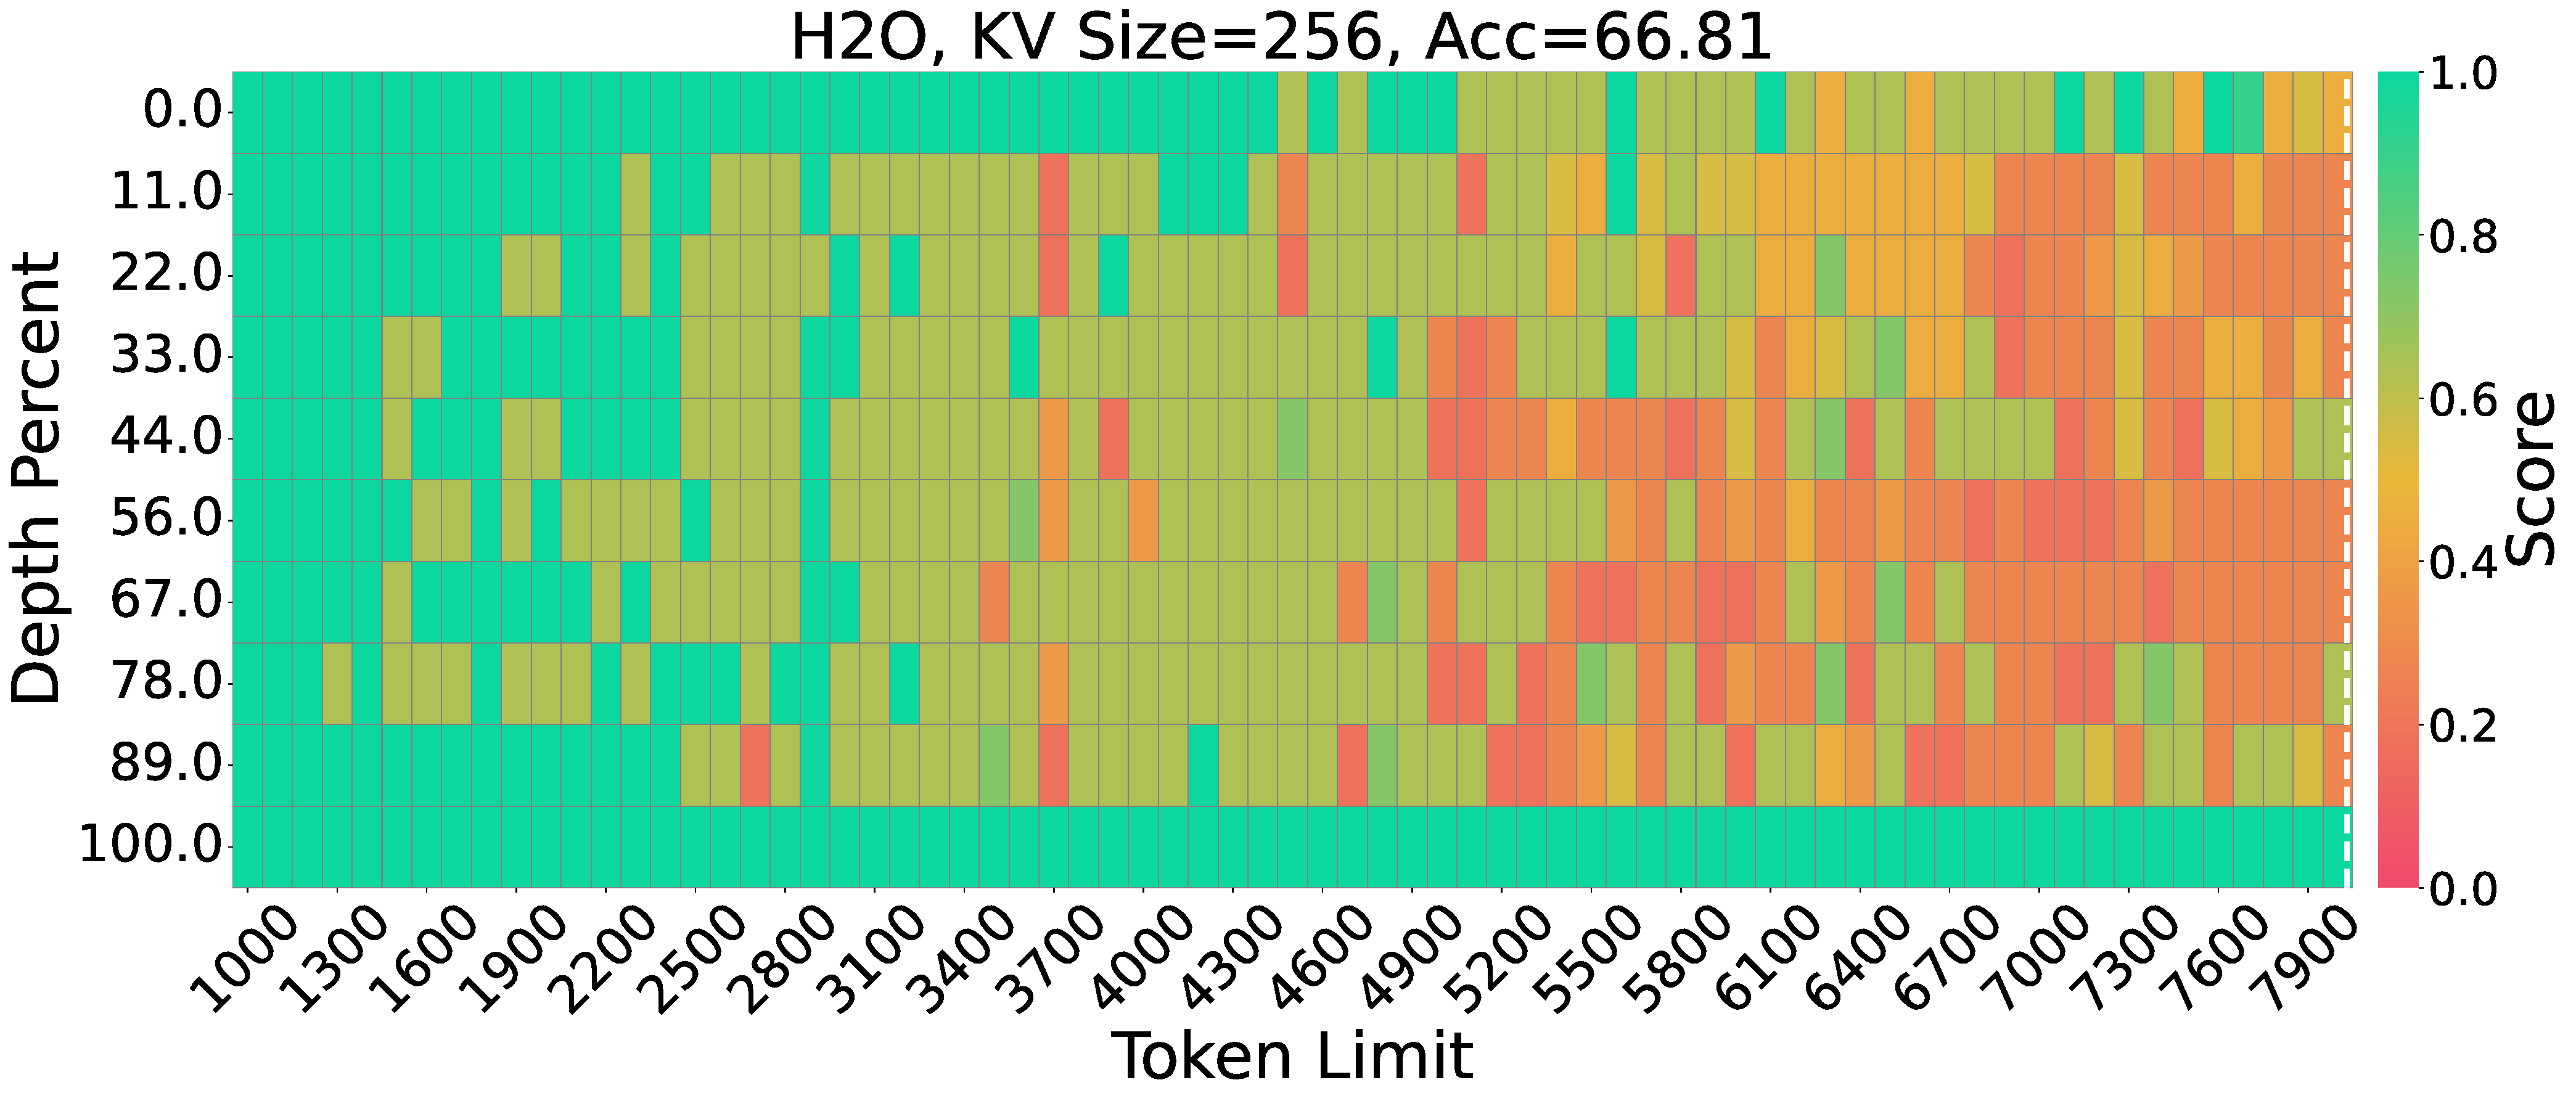
\includegraphics[width=\linewidth]{images/needle/llama-256/LlaMA3_h2o.pdf}
%     % \caption{H2O}
%   \end{subfigure}
%   \hfill
%   \begin{subfigure}[b]{0.48\linewidth}
%     \centering
%     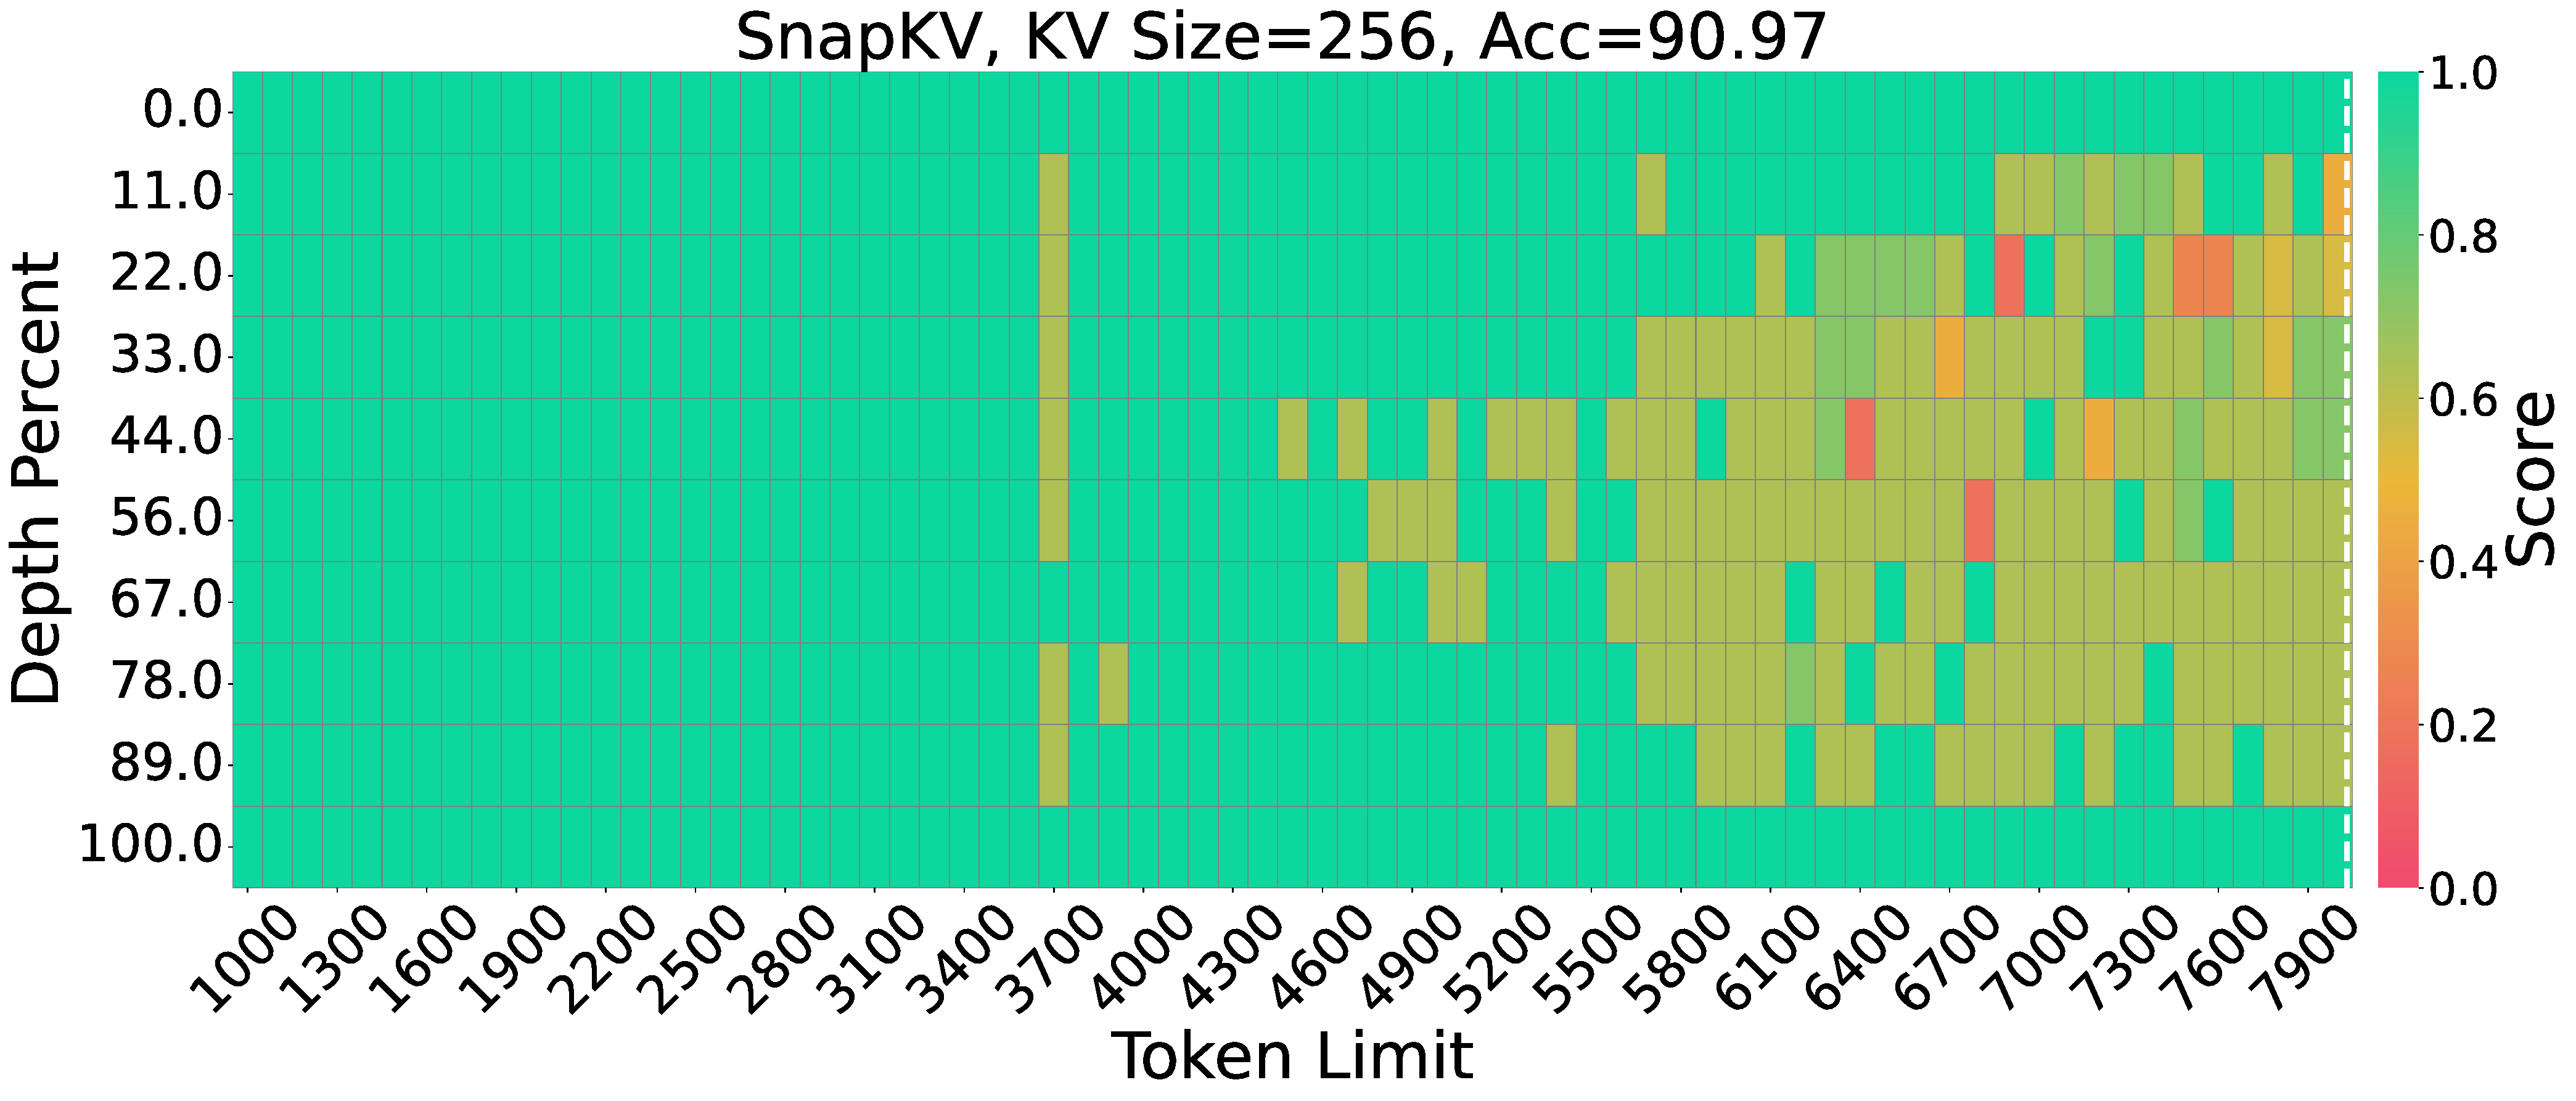
\includegraphics[width=\linewidth]{images/needle/llama-256/LlaMA3_snapkv.pdf}
%     % \caption{SnapKV}
%   \end{subfigure}
  
%   \vspace{0.1 cm}
  
%   \begin{subfigure}[b]{0.48\linewidth}
%     \centering
%     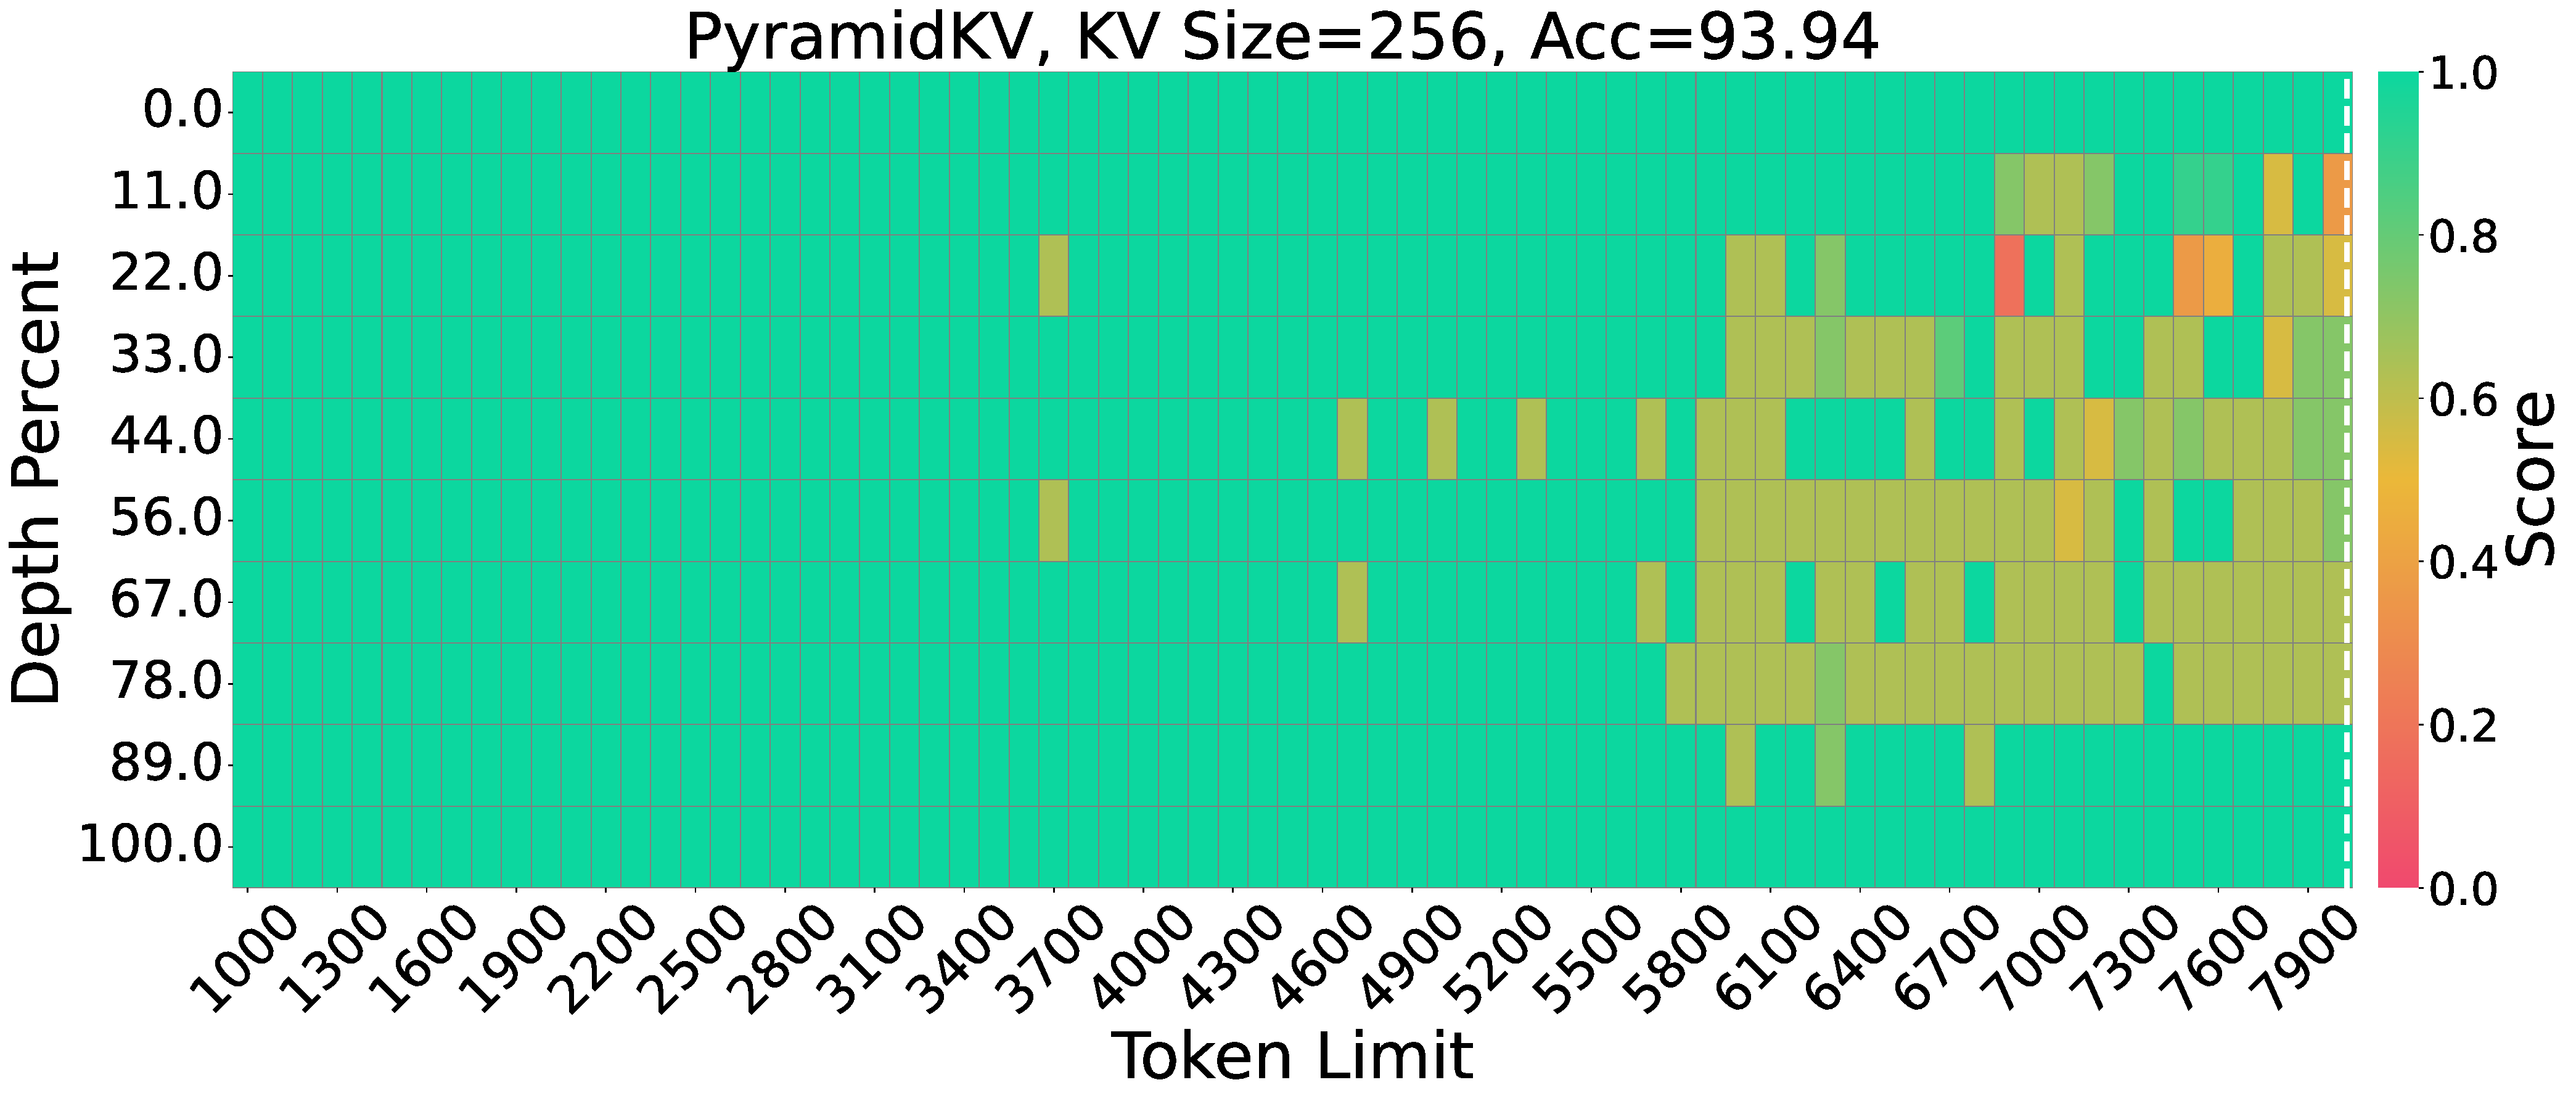
\includegraphics[width=\linewidth]{images/needle/llama-256/LlaMA3_pyramidkv.pdf}
%     % \caption{PyramidKV}
%   \end{subfigure}
%   \hfill
%   \begin{subfigure}[b]{0.48\linewidth}
%     \centering
%     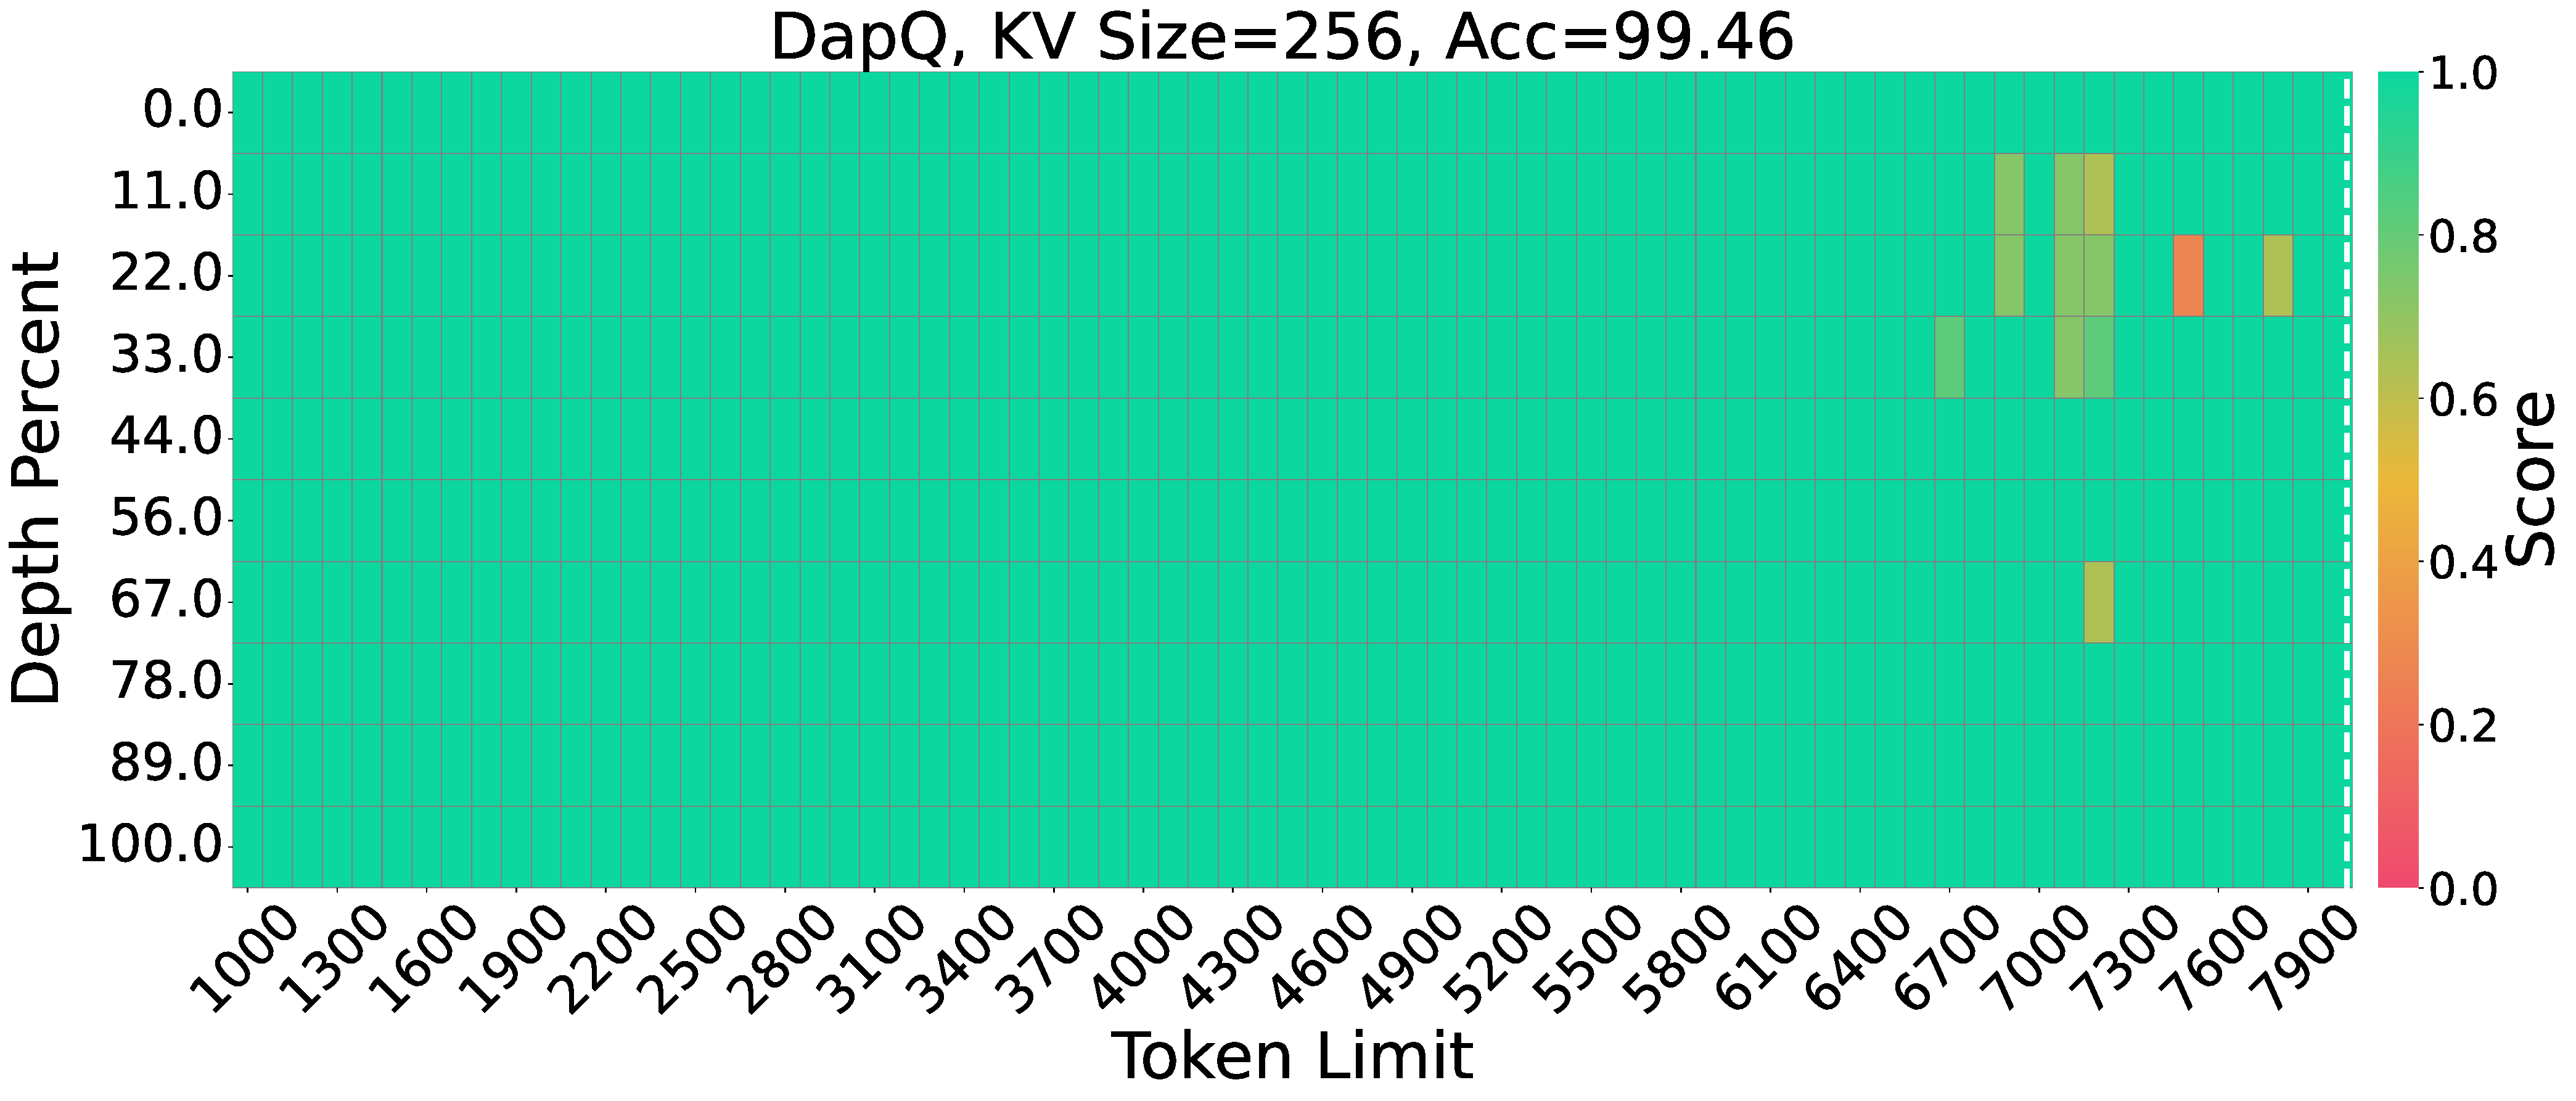
\includegraphics[width=\linewidth]{images/needle/llama-256/LlaMA3_ours.pdf}
%     % \caption{Ours}
%   \end{subfigure}
  
%   \caption{Results of Needle-in-a-Haystack on LLaMA-3-8B-Instruct with 8k context size and 256 KV size. The vertical axis of the figure represents the depth percentage, and the horizontal axis represents the token length.}
%   \vspace{-14pt}
%   \label{fig:needle}
% \end{figure*}


\begin{figure*}[t]
  \centering
  
  % 第一张图
  \begin{subfigure}[b]{0.7\linewidth} % 宽度设为0.7左右，居中显示
    \centering
    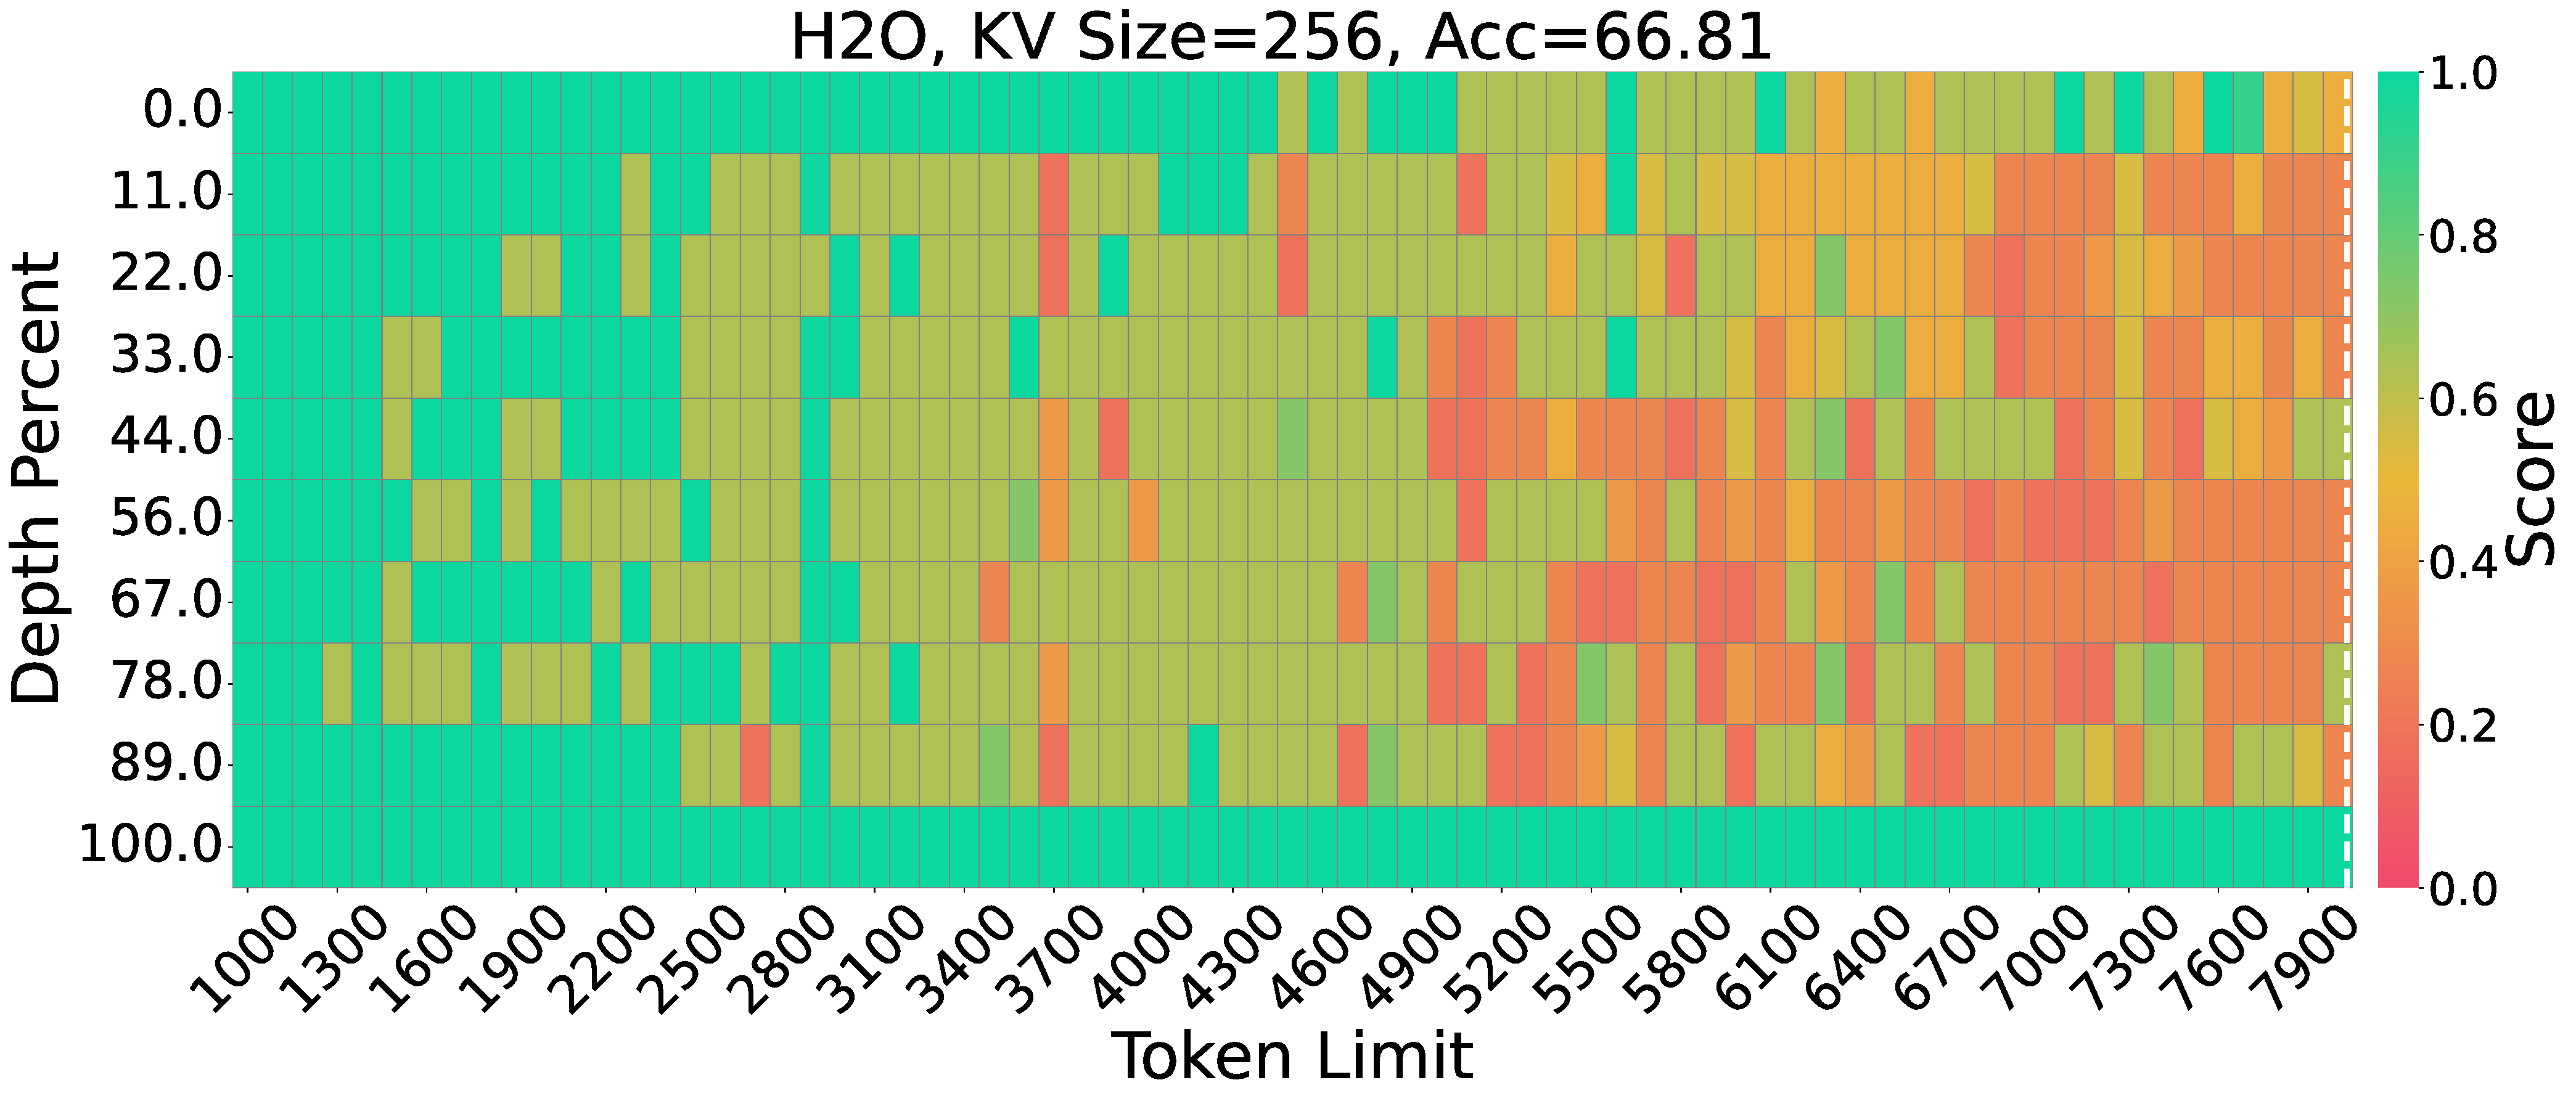
\includegraphics[width=\linewidth]{images/needle/llama-256/LlaMA3_h2o.pdf}
    % \caption{H2O}
  \end{subfigure}
  \par\vspace{0.2cm} % 【关键】强制换行 + 垂直间距
  
  % 第二张图
  \begin{subfigure}[b]{0.7\linewidth}
    \centering
    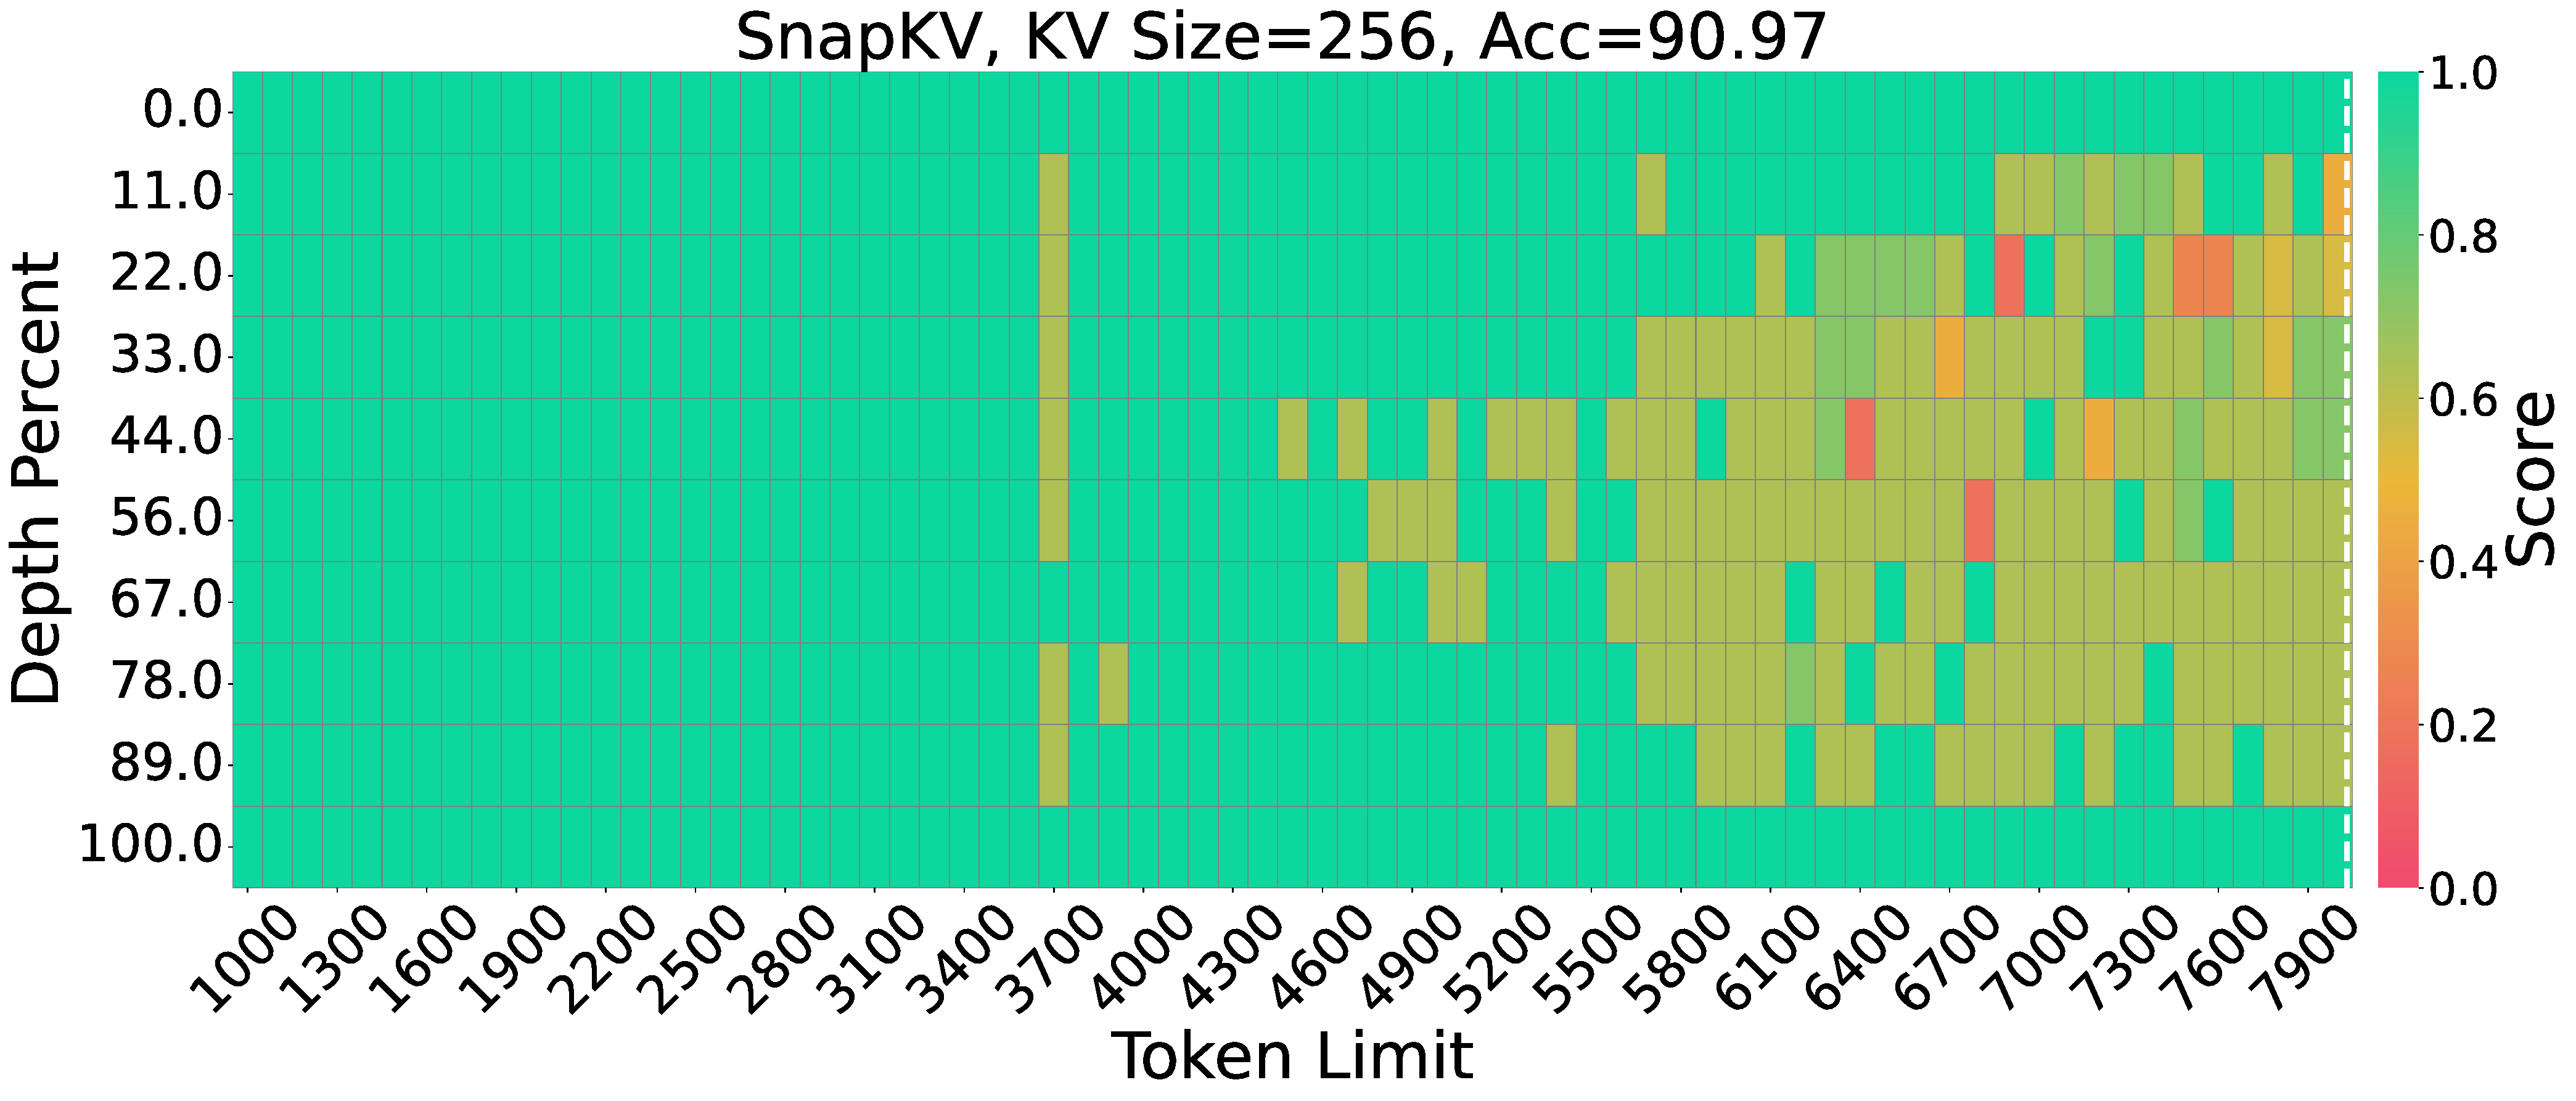
\includegraphics[width=\linewidth]{images/needle/llama-256/LlaMA3_snapkv.pdf}
    % \caption{SnapKV}
  \end{subfigure}
  \par\vspace{0.2cm}
  
  % 第三张图
  \begin{subfigure}[b]{0.7\linewidth}
    \centering
    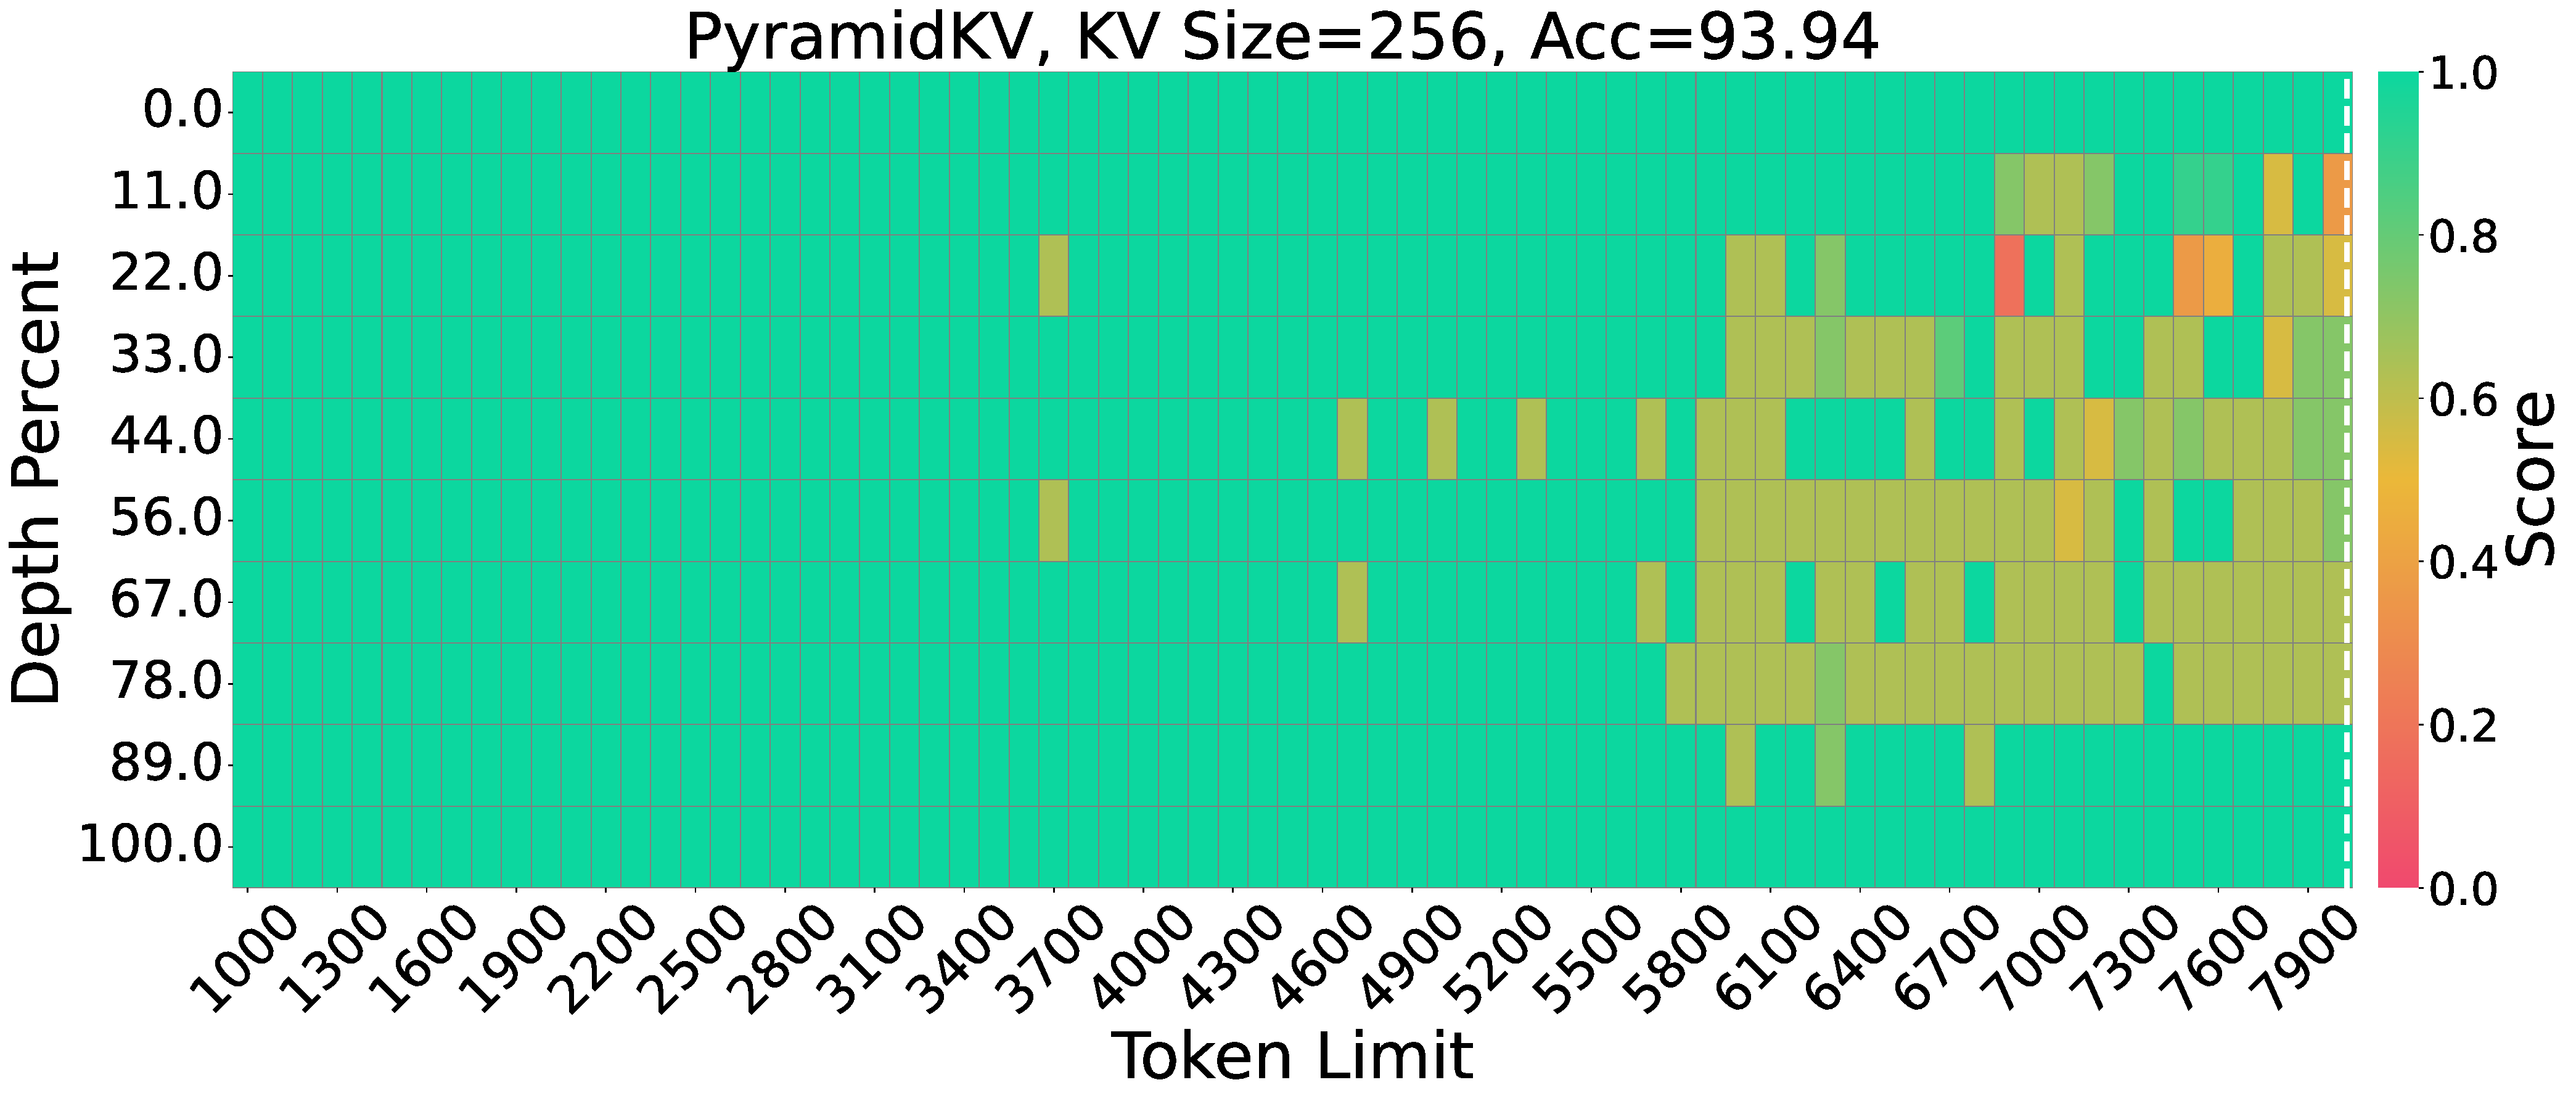
\includegraphics[width=\linewidth]{images/needle/llama-256/LlaMA3_pyramidkv.pdf}
    % \caption{PyramidKV}
  \end{subfigure}
  \par\vspace{0.2cm}
  
  % 第四张图
  \begin{subfigure}[b]{0.7\linewidth}
    \centering
    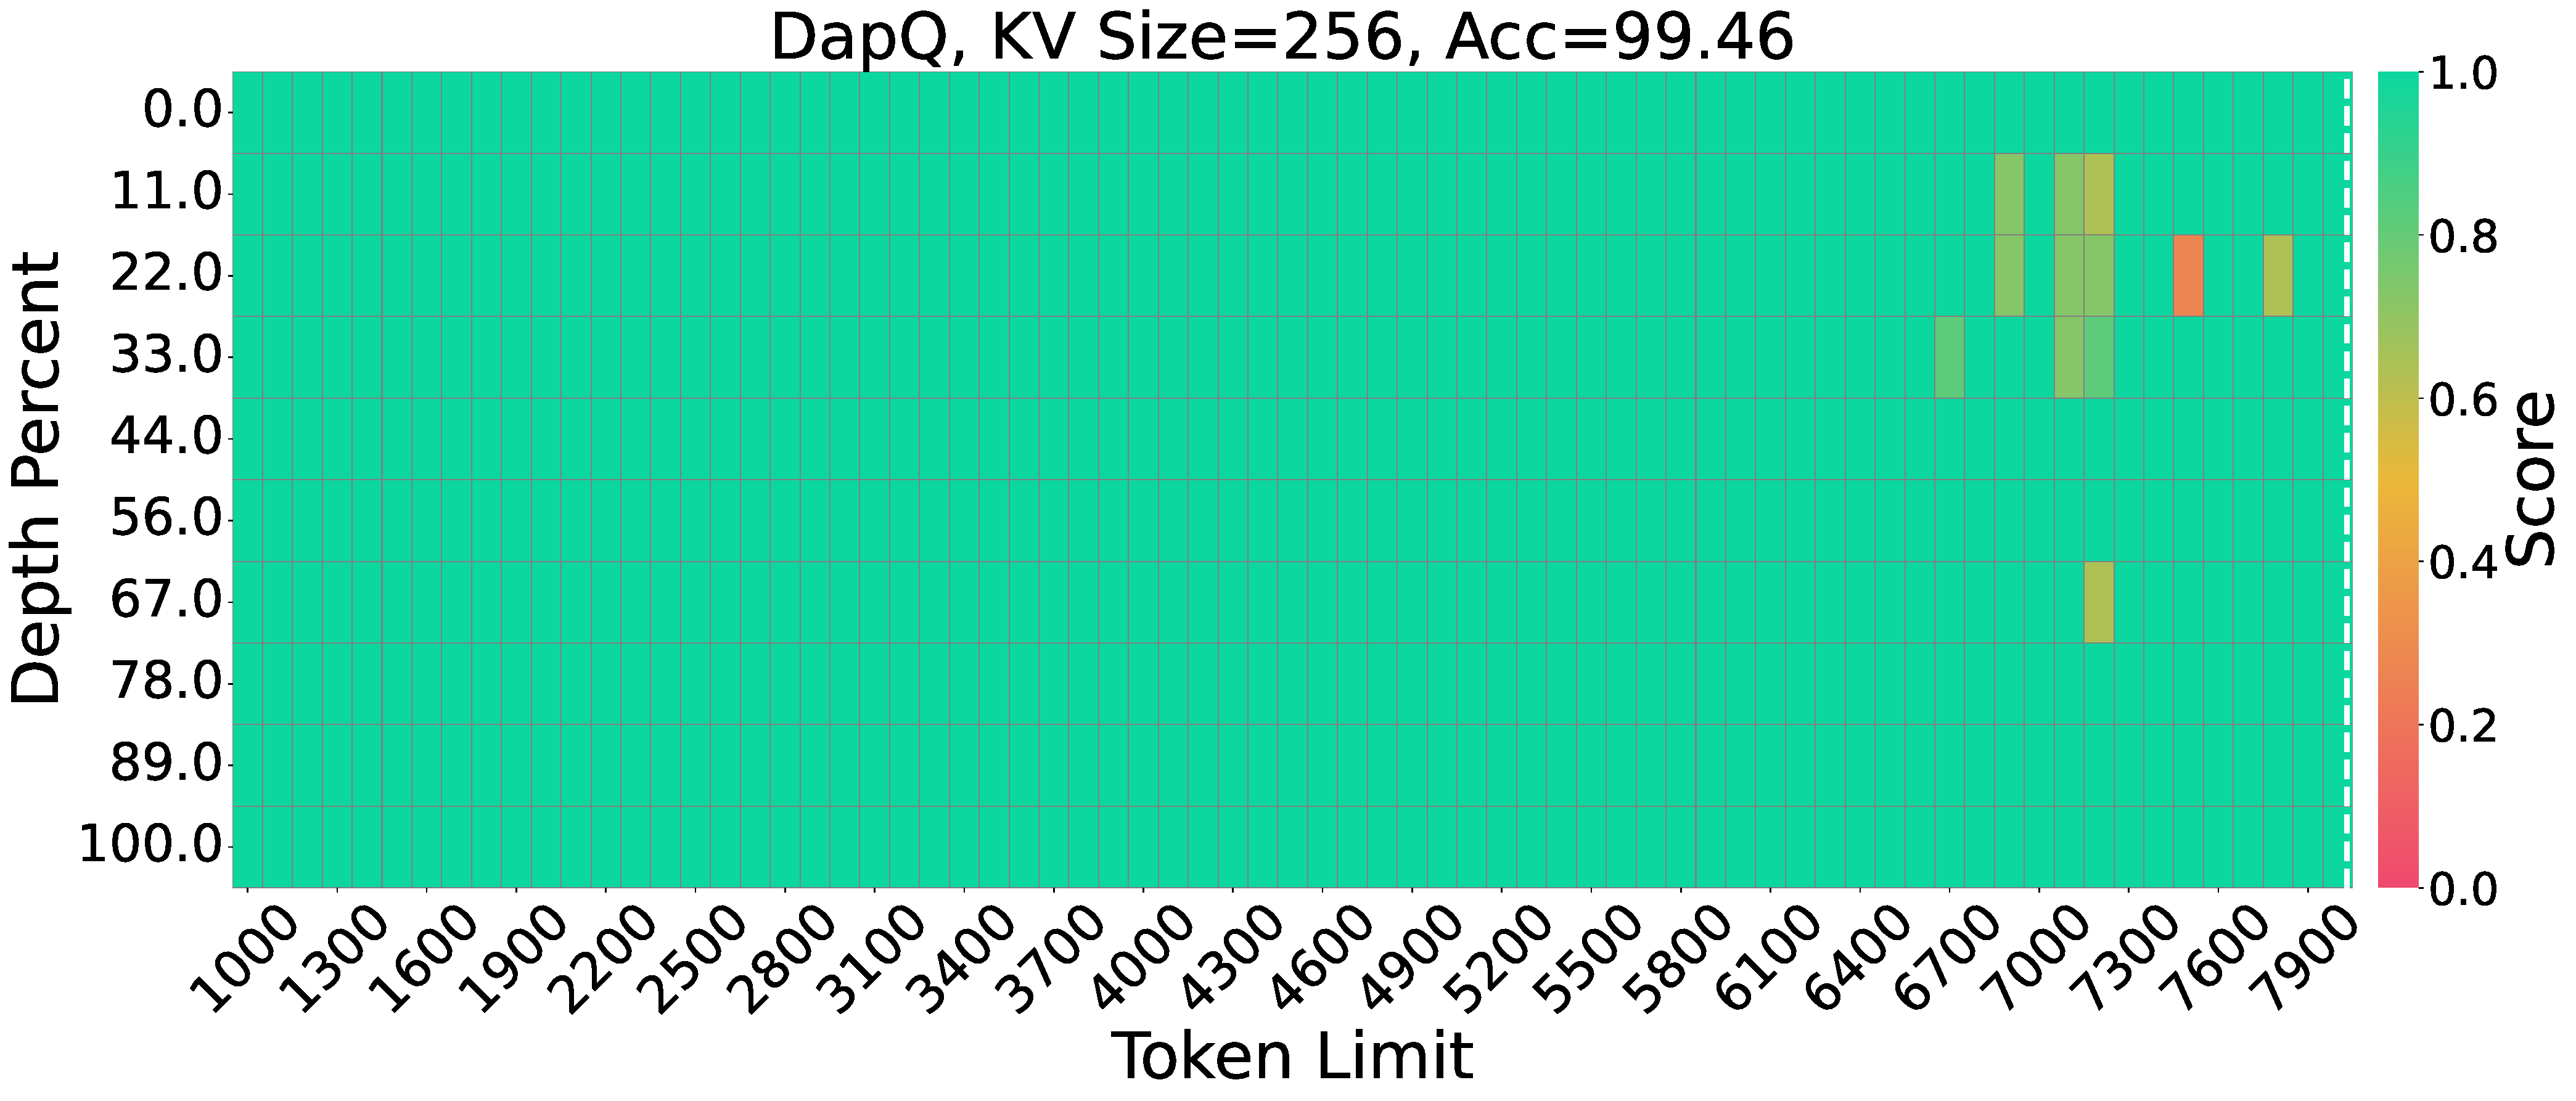
\includegraphics[width=\linewidth]{images/needle/llama-256/LlaMA3_ours.pdf}
    % \caption{Ours}
  \end{subfigure}
  
\caption{Visualization of Needle-in-a-Haystack results. We take LLaMA-3-8B-Instruct (8k context, 256 KV size) as a representative example to demonstrate the performance differences. The vertical axis represents the depth percentage, and the horizontal axis represents the token length.}
  \vspace{-14pt}
  \label{fig:needle}
\end{figure*}


\subsection{Improvement on Accuracy}
Consistent accuracy gains across benchmarks:
\textbf{LongBench Results.} As shown in Table \ref{table:longbench}, DapQ consistently outperforms all baselines across different models and cache budgets. The advantage is particularly pronounced under aggressive compression (e.g., budget=64), where DapQ shows a robust ability to retain critical information (e.g., preserving the long-range contextual dependencies especially on complex information integration tasks like HotpotQA and 2WikiMQA) and mitigate high-compression performance degradation. 
\textbf{LongBenchV2 Results.}
Under a 64 cache budget, DapQ achieves 29.26\% accuracy in the category of \enquote{Hard}, marking a +6.75\% absolute improvement over SnapKV (22.51\%) on LLaMA3-8B-Instruct.
\textbf{Ruler Results.}
Table \ref{table:ruler_llama3} shows that DapQ attains a notable 59.6\% accuracy on the challenging S-NIAH-3 task with a cache budget of 512, substantially outperforming SnapKV (1.4\%) and H2O (2.4\%). 
\textbf{HELMET Results.}
As reported in Table \ref{table:helmet}, DapQ achieves an average score of 48.10 on Qwen2.5-7B-Instruct with a low cache budget of 512, surpassing strong baselines SnapKV (43.74), H2O (40.36), and PyramidKV (42.49). 
\textbf{Needle-in-a-Haystack Results.}
As shown in Figure \ref{fig:needle} and Table \ref{table:needle}, a striking example is on LLaMA3-8B with a cache size of 256: DapQ achieves 99.5\% accuracy, closely approaching full-cache performance. This exceptional performance shows DapQ effectively simulates the decoding-stage positional context via prospectively encoded pseudo queries, enabling precise identification and retention of the key “needles” amidst a vast “haystack” of tokens.


Across diverse benchmarks, DapQ demonstrates the highest average score across nearly all budget settings on different models and especially delivers strong performance gains under strict cache constraints. These results underscores its effectiveness, robustness and generalizability in identifying and preserving critical contextual information. 




% \textbf{Ruler Results.} We further evaluate DapQ's reasoning capabilities under extreme memory constraints using the RULER benchmark, which tests models on synthetic long-context tasks including multi-hop tracing, retrieval, aggregation, and question answering. Under strict memory constraints, DaqQ exhibits a significant advantage. For instance, Table \ref{table:ruler_llama3} shows that on the Llama3-8B model with a cache budget of 512, DapQ achieves a notable 59.6\% accuracy in the challenging S-NIAH-3 task, substantially outperforming SnapKV (1.4\%) and H2O (2.4\%). This highlights its superior capability in preserving essential information necessary for complex tasks. Furthermore, DapQ consistently demonstrates the highest overall average score across nearly all budget settings on different models, underscoring its robustness and generalizability.


% \textbf{Needle-in-a-Haystack Result.} As shown in Figure \ref{fig:needle} and Table \ref{table:needle}, DapQ demonstrates universally superior performance compared to all baselines, confirming its consistent effectiveness. A striking example is on LLaMA3-8B with a cache size of 256: DapQ achieves 99.5\% accuracy, closely approaching full-cache performance. This exceptional performance shows its ability to maintain key contextual dependencies within constrained memory capacity. DapQ effectively simulates the decoding-stage positional context via prospectively encoded pseudo-queries, enabling precise identification and retention of the key “needles” amidst a vast “haystack” of tokens.

\subsection{Analysis on Efficiency}
We conduct a comprehensive efficiency evaluation of DapQ using Llama-3.1-8B-Instruct. We first focus on memory usage and throughput across different batch sizes (Input 8k, Output 150 tokens, Budget=256). As shown in Table \ref{tab:throughput_comparison} and Table \ref{tab:memory_comparison}, DapQ maintains robust performance, exhibiting memory and throughput highly on par with other compression methods. Furthermore, to assess the algorithmic overhead introduced during the prefill stage, we measure the Time-to-First-Token (TTFT) across varying sequence lengths from 8K to 128K. Table \ref{tab:ttft_comparison} indicates that the latency of DapQ is nearly identical to that of SnapKV. The results confirms that the additional prefill-stage overhead is almost negligible. Overall, DapQ achieves a balanced performance between long-context understanding capability and inference efficiency, ensuring its practicality for real-world long-context applications.









